\documentclass[12pt]{book}
\usepackage[nottoc,notlot,notlof]{tocbibind}
\usepackage[letterpaper]{geometry}
\geometry{left=2.5cm, right=2.5cm, top=2.5cm, bottom=2.5cm}
\usepackage[utf8]{inputenc}
\usepackage[spanish,mexico]{babel}
\usepackage{graphicx}
\usepackage[T1]{fontenc}
\usepackage{pslatex}


\title{
	
\includegraphics[width=0.8 \textwidth]{imagenes/logo} \\
	{\emph{\small FACULTAD DE INGENIERÍA ELECTROMECÁNICA }  } \\
	\vspace*{0.25in}
	\textsc{BOYA  ESTÁTICA PARA EL MONITOREO DE VARIABLES EN UN ENTORNO MARINO} \\
	
	{\Large Tesis para obtener el titulo de } \\
	\textbf{ \textbf{ {\large Ingeniero en Sistemas Computacionales} } } \\
	
	{\Large Presenta: } \\
	\textbf{ {\small Erik Alberto Mora Alvarez \\ Brenda Lourdes González De León } } \\
	{\Large Asesor: } \\
	\textbf{ \textbf{ {\large Verde Romero Daniel Alfonso} } } \\	
	{\Large Coasesor: } \\
	\textbf{ \textbf{ {\large Jiménez Betancourt Ramon Octavio} } } \\
	
 }
\date{Manzanillo, Colima, México, Junio de 2021}

\begin{document}
	
\maketitle
\frontmatter
\chapter*{Agradecimientos}
Agradecemos principalmente a nuestros padres por darnos todo el apoyo para poder llegar hasta este momento, también por creer en nosotros y aconsejarnos para seguir nuestros sueños y no darnos por vencidos, también a nuestro asesor por tomarse el tiempo para aconsejarnos y mejorar en el proyecto de tesis.

\chapter*{Resumen}
En el presente documento contiene una investigación acerca de la aplicacion del monitoreo  de variables de una boya estática que se localizará en la playa de manzanillo Colima. Cuenta con una página web donde se visualiza los datos obtenidos de los sensores en la boya que serán tomados de la placa sigfox que usamos por su cobertura, anteriormente la boya usaba red satelital pero el consumo de energía y costo se optó con este trabajo el uso de la tecnología sigfox por el menor costo, baja energía y fácil utilización además que proporciona localización del los dispositivos. Tiene como principal función proporcionar información de los sensores en tiempo real para uso externo de la universidad, permite interacción con la información de los sensores en el periodo de tiempo que seleccióne el usuario así como visualizar su localización. Por medio de la aplicación el usuario puede observar los datos de los sensores en cualquier fecha que desee y así mismo poder descargar la información en formato Excel para uso exclusivo de los usuarios.

\chapter*{Abstract}
This document contains an investigation about the application of variable monitoring of a static buoy that will be located on the Manzanillo Colima beach. It has a web page where the data obtained from the sensors on the buoy is displayed, which will be taken from the sigfox board that we use for its coverage, previously the buoy used a satellite network but the energy consumption and cost were chosen with this work. of sigfox technology due to the lower cost, low energy and easy use, in addition to providing location of the devices. Its main function is to provide information from the sensors in real time for external use of the university, it allows interaction with the information of the sensors in the period of time that the user selects as well as to visualize their location. Through the application, the user can observe the data from the sensors on any desired date and also be able to download the information in Excel format for the exclusive use of users.
\tableofcontents
\listoffigures
\mainmatter
\chapter{Introducción}
\section{Antecedentes}
En la actualidad vemos como cada vez más el uso del IoT gana terreno en nuestra vida cotidiana, ya que los proyectos que implementan esto cada vez son más, se sabe que desde hace tiempo existen tanto sistemas como dispositivos que nos facilitan las tareas, pero ahora tener un dispositivo con conexión a internet se ha vuelto más común, desde electrodomésticos hasta herramientas útiles para el trabajo, poder monitorear desde sensores hasta circuitos cerrados integrados en algún tipo de sistema. \\
\\
Kevin Ashton, cofundador del Auto-ID Center en MIT, mencionó por primera vez el internet de las cosas en una presentación que hizo a Procter \verb|&| Gamble (P\verb|&|G) en 1999. Queriendo que la ID de frecuencia de radio (RFID) llamara la atención de P\verb*|&|G la gerencia superior, Ashton llamó a su presentación “Internet de las cosas” para incorporar la nueva tendencia de 1999: internet. El libro del profesor del MIT, Neil Gershenfeld, When Things Start to Think, que apareció también en 1999, no utilizó el término exacto, pero proporcionó una visión clara de hacia dónde se dirigía IoT. \\

Un ecosistema de IoT consiste en dispositivos inteligentes habilitados para la web que utilizan procesadores integrados, sensores y hardware de comunicación para recopilar, enviar y actuar sobre los datos que adquieren de sus entornos. Los dispositivos de IoT comparten la información del sensor que recopilan al conectarse a una puerta de enlace de IoT u otro dispositivo de borde donde los datos se envían a la nube para analizarlos o analizarlos localmente. A veces, estos dispositivos se comunican con otros dispositivos relacionados y actúan sobre la información que obtienen unos de otros. Los dispositivos realizan la mayor parte del trabajo sin intervención humana, aunque las personas pueden interactuar con ellos, por ejemplo, para configurarlos, darles instrucciones o acceder a los datos.
Los protocolos de conectividad, redes y comunicación utilizados con estos dispositivos habilitados para la web dependen en gran medida de las aplicaciones específicas de IoT implementadas.
\vspace{10cm}
\subsection{Ventajas del IoT}
\begin{itemize}
	\item Monitorear sus procesos comerciales generales
	\item Mejorar la experiencia del cliente
	\item Ahorre tiempo y dinero
	\item Mejorar la productividad de los empleados
	\item Integrar y adaptar modelos de negocio
	\item Tomar mejores decisiones de negocios y
	generar más ingresos
\end{itemize}
La IoT alienta a las empresas a repensar las formas en que se acercan a sus negocios, industrias y mercados y les brinda las herramientas para mejorar sus estrategias comerciales.

\subsection{Boya Holbox-México}
La Comisión Nacional para el Conocimiento y Uso de la Biodiversidad (Conabio), en colaboración con la Secretaría de Marina (SEMAR), el CINVESTAV-Mérida del Instituto Politécnico Nacional, la Universidad Nacional Autónoma de México (Instituto de Ingeniería y el Centro de Ciencias de la Atmósfera), la Facultad de Ciencias Marinas de la Universidad Autónoma de Baja California en Ensenada (UABC-Ensenada), el Centro de Investigación Científica y de Educación Superior de Ensenada (CICESE) , la Secretaría de Medio Ambiente y Recursos Naturales (SEMARNAT) y la Comisión Nacional de Áreas Naturales Protegidas (CONANP), instalaron el 22 de julio de 2012, la boya oceánica Holbox-México para el monitoreo ambiental de parámetros oceanográficos, de calidad del agua y meteorológicos. El 7 de marzo de 2013 la boya quedó fuera de operaciones por robo de partes. El 16 de diciembre de 2015, con el apoyo de un buque de la SEMAR, se reinstala la Boya Holbox-México con los mismos sensores pero sobre una plataforma renovada. \\
Con esta estación de monitoreo ambiental se estudia el comportamiento espacio-temporal de las surgencias de Cabo Catoche y su conectividad con los eventos de florecimientos algales en el Banco de Campeche, creando capacidades para el monitoreo de ecosistemas marinos de México. Los datos calibrados obtenidos permiten validar las observaciones satelitales y tener insumos para la implementación del Sistema Satelital de Alerta Temprana de Florecimientos Algales, de apoyo a la toma de decisiones \cite{holbox}.

\section{Definición del problema}
Actualmente la boya que esta situada en FACIMAR tiene un sistema de sensores el cual se alimenta con una batería y anteriormente estaba conectada vía satélite, la conexión vía satélite actualmente tiene un alto costo agregando que tiene desventajas como la dependencia de las condiciones climáticas y una alta latencia para transmitir paquetes, ya que esto influye en las comunicaciones, para eso se integrara una tarjeta Sigfox la cual es una red de bajo consumo y es ideal para este proyecto pero que también tiene sus desventajas como lo puede ser el uso limitado de envío de datos.

\section{Justificación}
En este caso el tema de esta tesis se apega más al tipo de boya oceanográfica ya que el sistema con el que se cuenta tiene sensores para tomar medidas como son: la temperatura, la oxigenación y el dióxido de carbono tanto del mar como del aire y en el cual se tiene como propósito conectar mediante una red ese sistema integrado con el que cuenta la boya para poder enviar los datos que llega a tomar y así mostrarlos de forma visual al usuario para llevar el control de las diferentes variables que se toman en cuenta en el ambiente marino, para fines académicos o de investigación.

\section{Objetivos}
Los objetivos de esta tesis son varios, partiendo de la aplicación del IoT lo cual se puede aplicar para muchas otras cosas, en esta ocasión los objetivos a desarrollar son los siguientes:

\subsection{Objetivo general}

\begin{itemize}
	\item Diseñar una aplicación web en la cual se mostrarán de forma gráfica los datos enviados y una geolocalización de la boya.
\end{itemize}

\subsection{Objetivos especificos}

\begin{itemize}
	\item Enviar los datos de los sensores mediante la red Sigfox.
	\item Mostrar las diferentes variables que se toman de los sensores en tiempo real.
	\item Desarrollo de la documentación de los avances obtenidos.
\end{itemize}

Con esto se pretende tener un control y monitoreo de los datos que se registran día a día mediante las pruebas que va recolectando el sistema de la boya y mandar esos datos mediante Sigfox a una aplicación web para poder visualizarla de forma grafica y tener la localización de la misma de forma remota.


	
\chapter{Marco Teórico}

\section{Boyas Oceanográficas}
 Una boya es un objeto flotante situado en el mar para diversas finalidades, tales como señalización para la navegación o como estación meteorológica o incluso para detectar submarinos (usado en la guerra). Las boyas oceanograficas incorporan sistemas de adquisición de datos para obtener datos meteorológicos y oceanográficos de vital importancia.
 \begin{figure}[h]
 	\centering
 	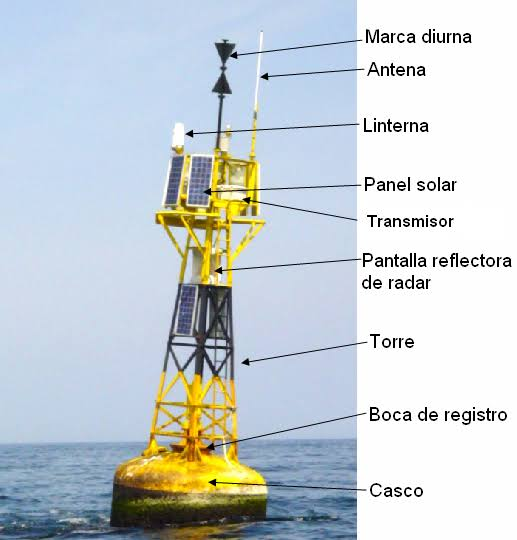
\includegraphics[width=0.5\linewidth]{imagenes/boya}
 	\caption[Boya Meteorológica ]{Boya Meteorológica}
 	\label{fig:boya}
 \end{figure}
\vspace{5cm}


\section{Tipos de boyas}

Las  Boyas estacionarias  se encuentran en una misma posición ancladas  en el fondo marino.Estas boyas cuentan con una superficie sumergida en el agua mientras que la otra parte es un mástil, los datos oceanográficos están localizados en la boya que se encuentra sujetada a una profundidad determinada en el cable de anclaje. Los datos meteorológicos se sitúan en el mástil a 2 metros. La recopilación de datos se compone por un sistema de adquisición, un sistema de comunicación inalámbrica y un equipo de recepción de datos. Las boyas disponen de unos paneles fotovoltaicos  que almacenan energía en las baterías para el funcionamiento de los equipos

Las Boyas Drifting miden datos oceanográficos puesto que su dimensión es muy pequeña, son lanzadas al mar para seguir las corrientes marinas para recopilar datos de interés. Su tiempo de vida es un minimo de 2 años, para ello disponen de un localizador GPS, un dispositivo de almacenamiento para extraer la información almacenada en ellas y cuentan con una batería que asegura su funcionalidad durante el tiempo de vida para la recopilación de datos.\cite{Tboyas}
  
\section{Variables Meteorologicas}
La meteorología abarca el estudio de los fenómenos físicos que ocurren en la atmósfera. Se puede conocer el estado del tiempo obteniendo información de algunas de sus variables. Las más útiles son las siguientes:
\subsection{ Viento}
El viento es el movimiento del aire. Según su intensidad y duración, pueden provocar pequeñas ráfagas de viento hasta tornados, por lo que es importante conocer la velocidad del viento y su dirección para prevenir catástrofes naturales.
Aunque también, para proporcionar información del viento a los navegantes. Para medir la velocidad del viento se usan los anemómetros. Estos pueden estar basados en diversos métodos de medida: de empuje, de rotación o de compresión, siendo el de rotación el más típico. Este método se basa unas cazoletas o hélices unidas a un eje central. El viento impacta sobre las cazoletas o hélices, de forma que hace rotar el eje central, produciendo una señal eléctrica con frecuencia proporcional a la velocidad del viento.
\subsection{Temperatura del aire}	

La temperatura es una propiedad física de la materia a la que nos referimos
como calor o ausencia de éste (frío). Así pues, la temperatura del aire sería el grado del calor específico.
El cuerpo humano percibe la temperatura del ambiente erróneamente al
mantener siempre el cuerpo a una temperatura constante, independientemente
de la exterior. Esto se llama sensación térmica. Para obtener una medida precisa de la temperatura de la atmósfera, se necesita utilizar el termómetro (cuyo significado es: medición de calor) y una escala para saber en qué valores de temperatura nos movemos. La temperatura se mide en grados diferentes según el país. Oficialmente, la unidad del SI es el Kelvin (K). Existen termómetros basados en diferentes principios, donde todavía se usan los métodos originales del termómetro hoy en día.
Principalmente se usan 2 métodos:
\begin{enumerate}
	\item La dilatación variable según la temperatura de un cuerpo sellado en un tubo. Una variación de temperatura provoca que el material se dilate más o menos, aumentando o disminuyendo el volumen ocupado en el tubo. Esto se visualiza en una escala dibujada en el tubo para tener referencias sobre la 	temperatura.
	\item Transducción de temperatura a electricidad. Algunos elementos varían sus 	propiedades eléctricas según la temperatura (termistores) u otros se combinan para provocar una fuerza electromotriz por el efecto de diferencial 	de temperatura (termopares).
\end{enumerate}


\section{Variables Oceanográficas}
La oceanografía estudia los procesos biológicos, geológicos, físicos y químicos que ocurren en los mares y océanos. Las boyas oceanográficas están centradas en realizar estudios de los procesos físicos y químicos, ya que los biológicos (organismos marinos) y geológicos no son necesarios para la navegación marítima, y con los otros procesos, se puede obtener información más útil.

\subsection{Temperatura del agua}
Para medir la temperatura del agua, también se utilizan termómetros. Puesto que el agua y el aire son masas con energía calorífica interna.
Para medir la temperatura del agua, como es una variable sencilla de medir, el sensor utilizado para las corrientes ya proporciona la información de la temperatura del agua.

\subsection{Oxígeno disuelto}

En los líquidos, podemos encontrar oxígeno en mayor o menor medida. Todo
líquido absorbe oxígeno hasta alcanzar una condición de equilibrio de presiones.
La concentración real de oxígeno disuelto depende de varios factores, como la temperatura, presión atmosférica, consumo y producción de oxígeno por los organismos. Por esto último, la concentración de oxígeno es importante para lavida de los peces y microorganismos en el agua.
Normalmente se utilizan dos escalas de medición: partes por millón (ppm); o porcentaje de saturación (\%), que se define como el porcentaje de oxígeno disuelto en 1 litro de agua, respecto la cantidad máxima de oxígeno disuelto que puede contener 1 litro de agua.
El sistema convencional de medición de oxígeno disuelto consiste en un medidor y una sonda polarográfica tipo Clark. La sonda es la parte más importante del sistema y la más delicada. La sonda consta de un ánodo de plata (Ag) revestido con un alambre de platino (Pt), que funciona como cátodo. Esto es insertado en una cubierta protectora llena de una solución electrolítica. La cubierta tiene en su extremo una membrana de Teflón, un material permeable al gas que permite elpaso del oxígeno presente en la solución, pero no el paso de la solución en sí.  \\ 
\\
\\
\subsection{Turbidez}
Se entiende por turbidez a la falta de transparencia en un líquido debido a la presencia de partículas. Cuanto más turbia esté el agua, más sucia parecerá, así que es usado como indicador para tener una estimación de la calidad del agua.
Existen dos formas de conocer la turbidez en un líquido: Según la absorción de la luz o la dispersión de la luz.
El primero se basa en proyectar un haz de luz con una longitud de onda determinada (casi en infrarrojo, pero tampoco en luz visible (700-1100 nm)),
para que las partículas sean las únicas capaces de atenuar esta luz. Esta atenuación de la luz servirá de indicador de la turbidez.
El segundo método, mide directamente la luz dispersada, en múltiples ángulos de medida. El medidor de turbidez detecta la luz dispersada por las partículas en suspensión en el agua, generando una tensión de salida proporcional a la turbidez o sólidos suspendidos.
\section{Tecnología Zigfox}
Sigfox es una tecnología de red de área amplia de baja potencia (LPWAN) especialmente diseñada para Internet de las cosas. Sigfox ofrece una solución de comunicaciones basada en software, donde toda la complejidad informática y de red se gestiona en la nube, en lugar de en los dispositivos. Todo eso junto, reduce drásticamente el consumo de energía y los costos de los dispositivos conectados. Su tecnología esta diseñada para cumplir con los requisitos de las aplicaciones de IoT, su batería cuenta con un amplio de vida y tiene una gran capacidad de red y lago alcance permitiendo adquirirla debido a su bajo costo.
\begin{figure}[h]
	\centering
	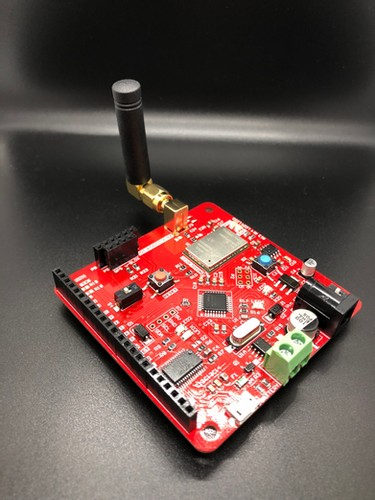
\includegraphics[width=0.4\linewidth]{imagenes/file}
	\caption[Tarjeta de Desarrollo Sigfox]{Tarjeta de Desarrollo Sigfox}
	\label{fig:file}
\end{figure}
\vspace{10cm}

\subsection{Características de Sigfox}
\begin{itemize}
	\item Autonomía: Consumo de energía extremadamente bajo, lo que permite años de duración de la batería.
	\item Sencillez: Sin configuración, solicitud de conexión señalización y el dispositivo funciona en minutos con una suscripción anual por dispositivo
	\item Eficiencia de costo. Desde el hardware utilizado en los dispositivos hasta nuestra red, optimizamos cada paso para que sea lo más rentable posible.
	\item Distancia: Puede variar dependiendo de los obstáculos pero podemos definirla entre 1-5 kilómetros en áreas urbanas densas, hasta 15-30 kilómetros en áreas rurales.
	\item Cobertura: Sigfox no solo se limito a lograr grandes distancias sino también una cobertura de alta densidad que permite conectar alrededor de 250,000 dispositivos por antena.
\end{itemize}
\subsection{Modo de Operación de Sigfox}
Sigfox transportan datos desde donde se encuentren instalados y hasta sus sistemas de TI para la visualización de los mismos, mediante el uso de antenas instaladas en lugares estratégicos en una determinada área y recibe datos de dispositivos (sensores en parquímetros, sensores de temperatura, medidores de luz eléctrica, medidores de agua etc.). 
Los dispositivos utilizan frecuencias de banda ISM sin licencia, es decir, 920 MHz (Sur América) u 868 MHz (Europa). En el caso de Norte América que es donde pertenece México manejamos una frecuencia de 902 Mhz, en la siguiente figura podemos ver la clasificación de las configuraciones de radio o RC (Radio Configurations) destinadas para los países donde se encuentra trabajando la red Sigfox.
\begin{figure}[h]
	\centering
	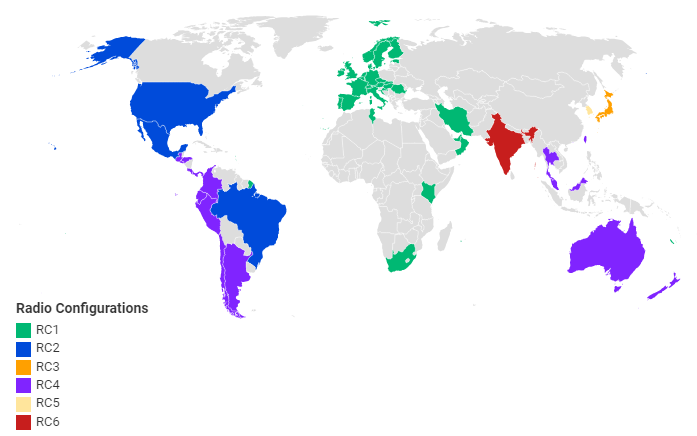
\includegraphics[width=0.8\linewidth]{imagenes/redsigfox}
	\caption[Países que cuentan con red Sigfox.]{Países que cuentan con red Sigfox.}
	\label{fig:redsigfox}
\end{figure} \\
Las tramas contienen un preámbulo de símbolos predefinidos utilizados para la sincronización en la transmisión. Los campos de sincronización de trama especifican los tipos de tramas que se transmiten. El FCS es una secuencia de verificación de trama (FCS – Frame Check Sequence) utilizada para la detección de errores. Ningún paquete contiene una dirección de destino u otro nodo. Todas las puertas de enlace (antenas) enviarán todos los mensajes al servicio en la nube (Backend) de Sigfox, estos mensajes son llamados Uplink. El mensaje que vemos en el recuadro rojo de la siguiente figura nos interesa que sea enviado, tiene su lugar en el campo llamado payload con un tamaño de 0 a 12 Bytes hexadecimales, el payload contiene las variables que estamos monitoreando en nuestra aplicación.
\begin{figure}[h]
	\centering
	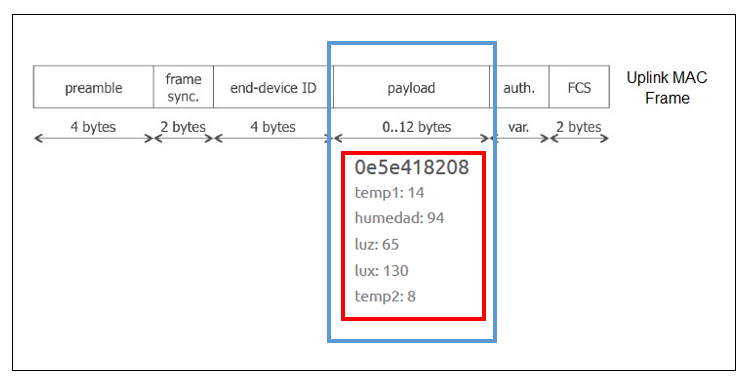
\includegraphics[width=0.7\linewidth]{imagenes/trama}
	\caption[Trama del mensaje enviado al Backend Sigfox. ]{Trama del mensaje enviado al Backend Sigfox. }
	\label{fig:trama}
\end{figure}

\subsection{Cobertura Sigfox en Manzanillo}
\begin{figure}[h]
	\centering
	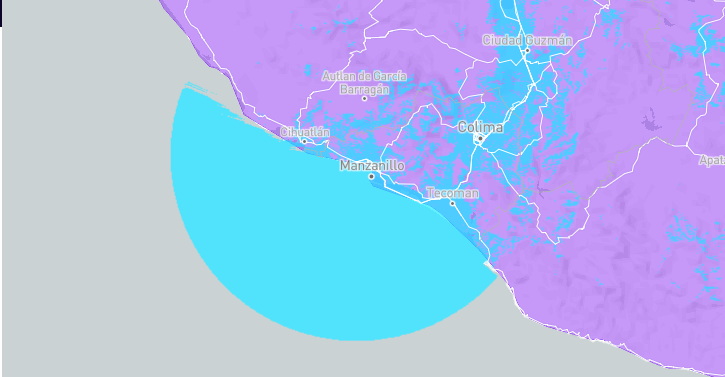
\includegraphics[width=0.8\linewidth]{imagenes/Cobertura}
	\caption{Cobertura de Sigfox en Manzanillo.}
	\label{fig:Cobertura de Sigfox en Manzanillo}
\end{figure}



\subsection{Backend de Sigfox}
El sigfox Backend es una comunicación que recibe los mensajes y los procesa para generar un resultado donde se pueden gestionar los dispositivos, visualizar los mensajes transmitidos por los mismos y configurar de integración de los datos, entre otros. Además, el servicio da la oportunidad de poder redirigir todo el volumen de información que llega al backend a cualquier aplicación ejecutada en un servidor o centro de procesamiento de datos.
Existen dos maneras de tomar los datos que recoge el backend de Sigfox:
\begin{itemize}
	\item Utilizando la API que proporciona el backend, basada en HTTP REST (GET o POST, indistintamente); la cual, en función del recurso pedido, devuelve un resultado concreto, con una carga útil con formato JSON.
	\item Utilizando una URL de callback, identificando dicha URL a la aplicación web que desea recibir los mensajes. De esta forma, se registraría dicha URL en el backend, indicando los atributos que le interese recibir (por ejemplo, la carga útil del mensaje); y cada vez que llegase un mensaje al mismo, éste le reenviará los valores pedidos en un mensaje con formato, por ejemplo JSON.
\end{itemize}
\subsection{Conectividad de Enlace Ascendente}
Los mensajes de radio emitidos por los dispositivos conectados son recolectados por las estaciones base de Sigfox, luego transmitidos a la nube de Sigfox y enviados a la plataforma de TI del usuario final. Cuenta con una red en estrella que permite transmitir mensajes or cualquier base en el rango.

\subsection{Pequeña carga Util }
Un mensaje de enlace ascendente tiene una carga útil de hasta 12 bytes y tarda un promedio de 2 segundos en llegar a las estaciones base que monitorean el espectro en busca de señales UNB para demodular. Para una carga útil de datos de 12 bytes, una trama Sigfox utilizará 26 bytes en total. La carga útil permitida en los mensajes de enlace descendente es de 8 bytes.
\subsection{Modulación de Radio de Banda Estrecha}
Usando la modulación de Banda Ultra Estrecha, Sigfox opera en los 200 kHz de la banda disponible públicamente para intercambiar mensajes de radio por aire. Cada mensaje tiene un ancho de 100 Hz y se transfiere a una velocidad de datos de 100 o 600 bits por segundo, según la región. Por lo tanto, se pueden lograr largas distancias siendo muy robusto contra el ruido.\cite{Sigfox} \\
\\
\\
\subsection{Funcionamiento}
Tiene un sistema en la nube donde desde la interfaz web es posible dar de alta los equipos, que funcionan por un ID único en vez de autenticación por tarjeta SIM como los móviles u otros dispositivos IoT basados en GPRS.
También ofrece una red con buena calidad de servicio garantizada y efectiva para bajo volumen de datos, pero que puede soportar muchos dispositivos simultáneos como por ejemplo un despliegue de sensores.

Podemos desarrollar nuestra propia APP y conectarla a la API de Sigfox para recibir la información de los sensores y dispositivos.
\begin{figure}[h]
	\centering
	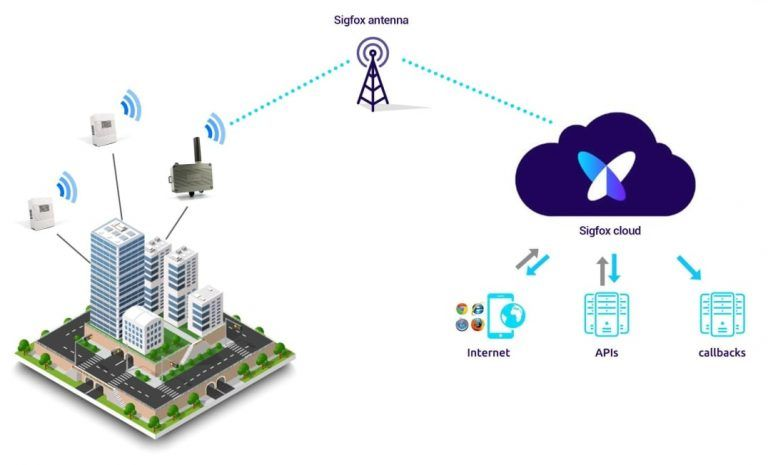
\includegraphics[width=0.5\linewidth]{imagenes/esquemasigfox}
	\caption[funcionamiento sigfox ]{Esquema de funcionamiento de sigfox}
	\label{fig:esquema}
\end{figure}
\vspace{10cm}



\section{Sensores}

Un sensor es un dispositivo que detecta el cambio en el entorno y responde a alguna salida en el otro sistema. Un sensor convierte un fenómeno físico en un voltaje analógico medible (o, a veces, una señal digital) convertido en una pantalla legible para humanos o transmitida para lectura o procesamiento adicional. \\

Los sensores se usan en nuestra vida cotidiana. Por ejemplo, el termómetro de mercurio común es un tipo de sensor muy antiguo utilizado para medir la temperatura. Usando mercurio coloreado en un tubo cerrado, se basa en el hecho de que este producto químico tiene una reacción constante y lineal a los cambios de temperatura. \\

\begin{figure}[h]
	\centering
	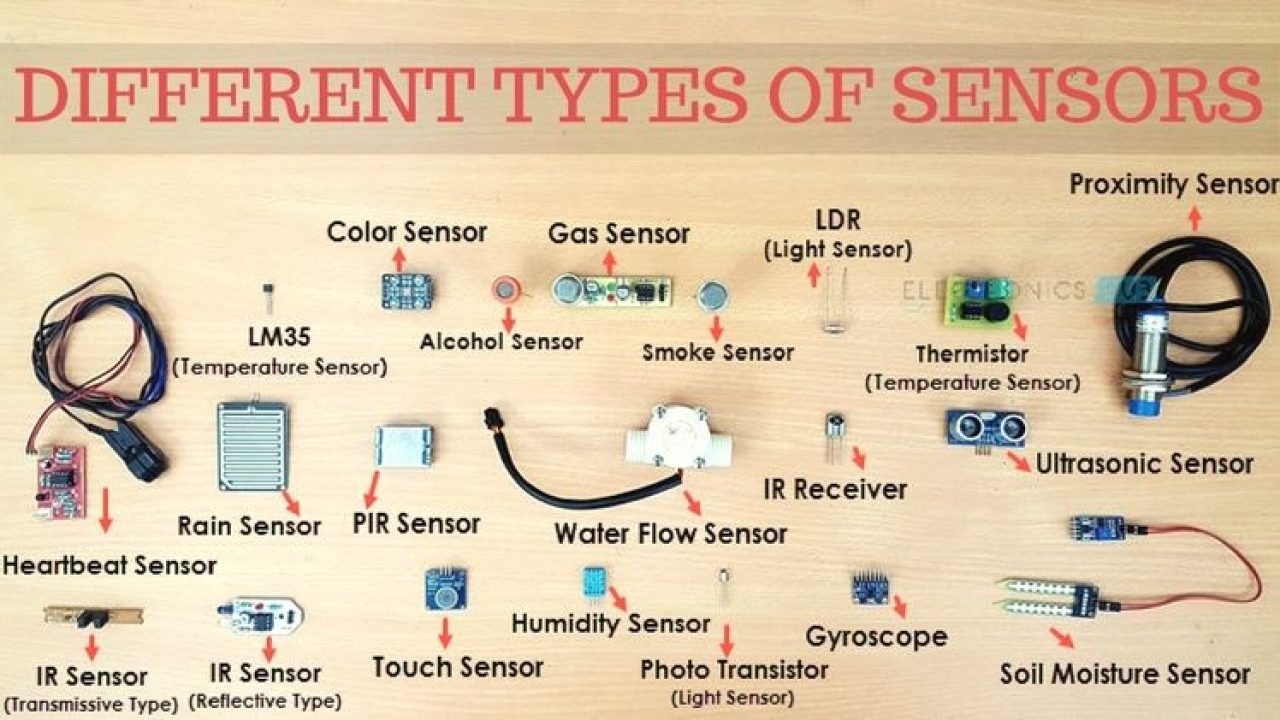
\includegraphics[width=0.6\linewidth]{imagenes/sensores}
	\caption[Sensores]{Sensores.}
	\label{fig:sensores}
\end{figure}

\vspace{4cm}


\subsection{Sensores de temperatura}

Un sensor de temperatura es un componente electrónico que devuelve una señal eléctrica que depende de la temperatura del sensor. A partir de la señal eléctrica se puede conocer la temperatura real a la que se encuentra el sensor. \\
Existen muchos tipos diferentes de sensores de temperatura. Cada tipo de sensor se adapta bien a una aplicación concreta. En estas prácticas se van a estudiar solo sensores de bajo precio que alcanzan un rango de temperaturas moderado, de -40ºC hasta 150ºC. Con una exactitud moderada, desde 1ºC hasta 0.1ºC de error. Los sensores de temperatura son muy útiles para construir aparatos de medida de temperatura y máquinas que regulan de forma automática la temperatura. \\

Algunos ejemplos en donde se hacen uso de los sensores de temperatura:
\begin{itemize}
	\item Termómetro digital para medir la temperatura del cuerpo.
	\item Termostato digital de una casa.
	\item Termostato de temperatura de un horno.
	\item Sensor de incendios.
	\item Termostato de acuario o de terrario.
	\item Termómetro digital de temperatura ambiente.
\end{itemize}
\subsubsection{Funcionamiento de un sensor NTC}

Una resistencia NTC es un componente que reduce su resistencia cuando aumenta la temperatura. Este sensor no es lineal. Esto quiere decir que su exactitud no es muy buena en rangos amplios de temperatura, comparada con otros sensores. A pesar de eso un sensor NTC bien ajustado puede medir temperaturas con bastante exactitud, 0.1ºC en un intervalo pequeño de temperaturas. \\
 \begin{figure}[h]
 	\centering
 	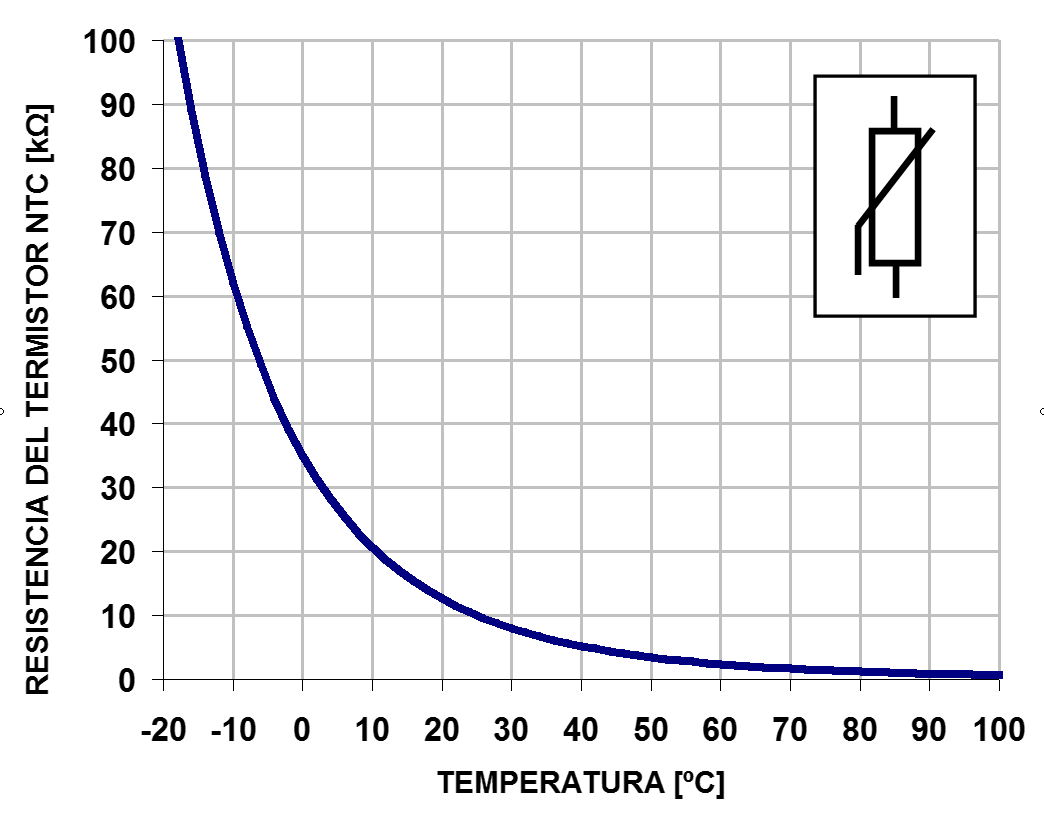
\includegraphics[width=0.4\linewidth]{imagenes/temperatura}
 	\caption[Grafica de rango de medición de temperatura]{Grafica de rango de medición de temperatura.}
 	\label{fig:temperatura}
 \end{figure}

 La resistencia disminuye a medida que aumenta la temperatura. La forma de la curva es no lineal, lo que da problemas a la hora de calcular con exactitud la temperatura.
 \subsection{Sensores de dióxido de carbono}
 
 Un sensor de CO2 es un instrumento que se utiliza para la medición de gas de dióxido de carbono en un ambiente determinado. Habitualmente estos aparatos registran el dióxido de carbono en partes por millón (ppm) en los espacios ocupados y nos ofrecen una muestra de la concentración de este gas en el aire que respiramos. Con la utilización de sensores de CO2 se pueden identificar las zonas o estancias habitadas en las que los niveles de dióxido de carbono son superiores a los aceptables. \\
 
 \begin{figure}[h]
 	\centering
 	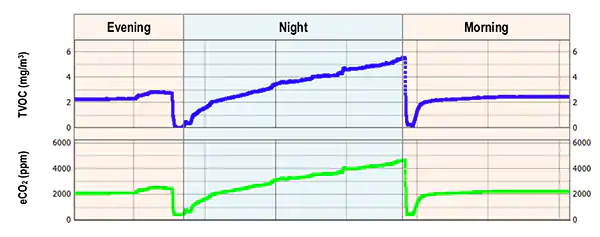
\includegraphics[width=0.6\linewidth]{imagenes/co2}
 	\caption[Grafica de rango de medición de CO2]{Grafica de rango de medición de CO2.}
 	\label{fig:co2}
 \end{figure}
 \subsubsection{Características de los sensores de CO2}
 \begin{itemize}
 	\item Son muy estables y altamente selectivos del gas medido
 	\item Se instalan fácilmente
 	\item Soportan condiciones de humedad alta, polvo, etc.
 	\item Tienen una prolongada vida útil
 \end{itemize}
En el momento de su instalación será conveniente tener en cuenta una serie de factores: el tipo de estancia y su geometría, su ocupación y la ventilación del área. Además, en determinados centros de trabajo donde la exposición al CO2 puede ser mayor, será aconsejable instalar los sensores cerca de los potenciales puntos de origen de las fugas para permitir una detección temprana.
\newpage
\subsection{Ruta Óptica LI-820}
El reflector y la trayectoria óptica están chapados en oro. para aumentar la transmisión de energía. El CO2 se mide en una única ruta a través del uso de filtros ópticos de banda estrecha. 
Un transductor de presión reduce la variabilidad debido a cambios en la presión barométrica. Un recinto de espuma rodea el banco óptico. Esto ayuda a mantener un entorno térmico controlado.
\begin{figure}[h]
	\centering
	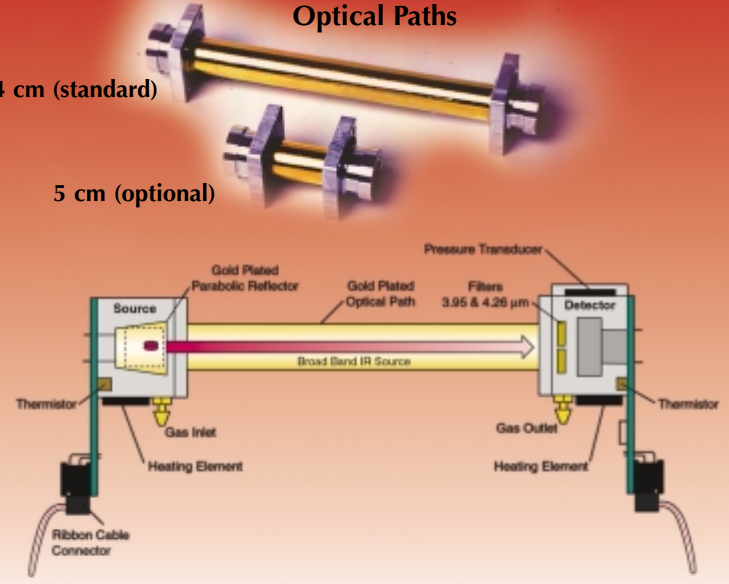
\includegraphics[width=0.4\linewidth]{imagenes/ruta}
	\caption[Ruta óptica LI-820 ]{Ruta Óptica}
	\label{fig:rutaoptica}
\end{figure}

 \subsection{Analizador CO2}
 Analizador de gases infrarrojo absoluto no dispersivo (NDIR) basado en detección de infrarrojos de una sola ruta y longitud de onda dual sistema, permite la monitorización continua de CO2.
 \begin{figure}[h]
 	\centering
 	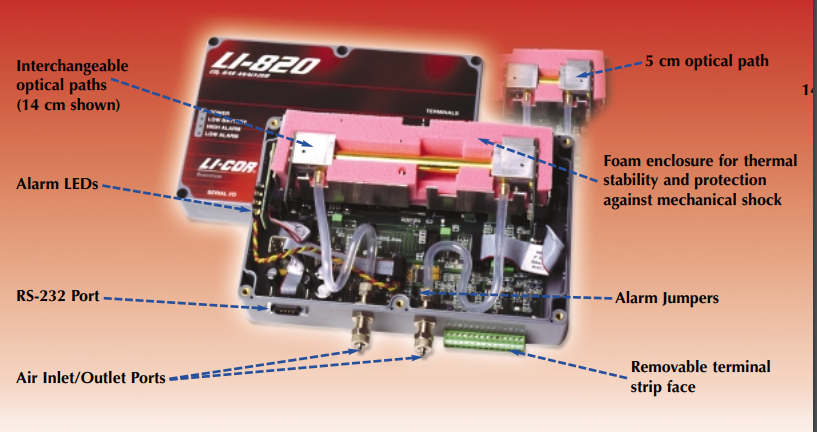
\includegraphics[width=0.4\linewidth]{imagenes/analizador}
 	\caption[Analizador de CO2 LI-820 ]{Analizador de CO2 }
 	\label{fig:analizador}
 \end{figure}//
\vspace{10cm}
\section{Internet de las cosas Subacuáticas (IoUWT)}
Internet de las cosas (IoT) que combina avances en
tecnologías de detección, computación móvil y servidor en la nube
y las plataformas se han vuelto muy importantes en los últimos años
importante y omnipresente en el mundo moderno. Como más
y se implementan más aplicaciones utilizando tecnologías de IoT,
la fragmentación de las tecnologías de IoT de propósito general para
dirigirse a sectores particulares con diferentes requisitos
ing necesario. \cite{IoT} \\
El Internet de las cosas submarino (UIoT), una extensión del Internet de las cosas (IoT) al entorno submarino, constituye una tecnología poderosa para lograr el océano inteligente. La UIoT está habilitada por los desarrollos más recientes en vehículos submarinos autónomos, sensores inteligentes, tecnologías de comunicación submarina y protocolos de enrutamiento submarino. En los próximos años, se espera que UIoT conecte diversas tecnologías para detectar el océano, lo que le permitirá convertirse en una red inteligente de objetos submarinos interconectados que tenga capacidades de autoaprendizaje y computación inteligente. \cite{UIoT}\\
Algunos desafíos adicionales para el IoUWT: (1) Eficiencia energética y dificultad para recargar. Debido a los altos costos de implementación de los sensores subacuáticos y la dificultad para recargar los dispositivos, la eficiencia energética es un desafío importante para IoUWT; (2) Cambios en la red topología debido al movimiento de los sensores submarinos; y (3) Inestable y baja confiabilidad debido a la pérdida de transmisión del
las señales acústicas son absorbidas por el medio acuático. \cite{Desafios}
\chapter{Metodología }

Para este proyecto de tesis se utilizara el modelo en cascada ya que este modelo se adapta al proceso de desarrollo que se llevara a cabo para esta tesis, partiendo desde los requisitos y el análisis del problema para tener una idea clara de lo que se va a resolver y después diseñar un sistema que se adapte para resolverlo, que en este caso consiste en desarrollar un sistema en el cual el usuario podrá visualizar en una interfaz de manera gráfica los diferentes datos que el servicio de Sigfox envía desde la tarjeta conectada a los sensores de la boya, para después implementarlo en un entorno real y hacer pruebas del comportamiento que toma y un análisis de los resultados. 

\begin{figure}[h]
	\centering
	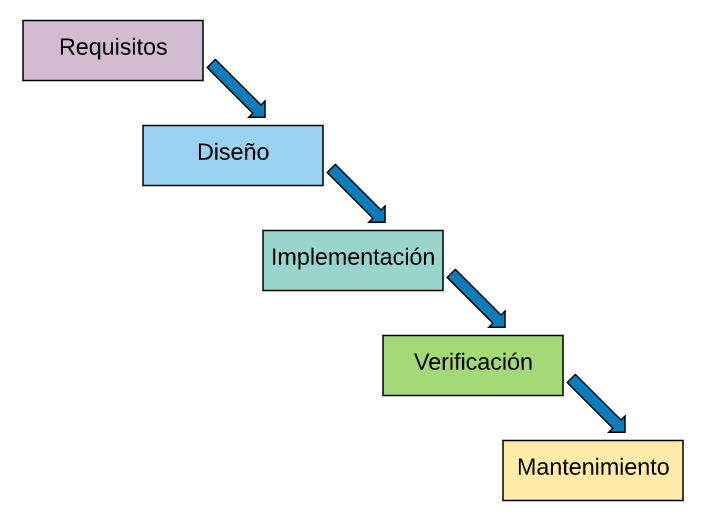
\includegraphics[width=0.5\textwidth]{imagenes/cascada}
	\caption[Modelo en cascada]{Modelo en cascada.}
	\label{fig:cascada}
\end{figure}

\section{Requisitos}
En esta etapa se investiga todo respecto al tema, en el caso de este proyecto, la investigación va desde el funcionamiento de la tarjeta y servicio Sigfox y como es que maneja él envió de datos, también entender el funcionamiento de una boya y el sistema de sensores que se manejan en ese tipo de boyas, para que son usados y con que fin se implementan en el entorno marino.

\section{Diseño}
En la etapa de diseño, se empieza por definir que es lo que se mostrara, en este caso la interfaz constara de una vista principal, en la cual mostrara las diferentes variables tomadas de los sensores, que en este caso son 4, oxigeno, dióxido de carbono , turbidez y temperatura, cada uno mostrando mediante un medidor, el dato que va cambiando constantemente, dependiendo si este se mantiene o cambia constantemente, también una sección donde se pretende que se pueda visualizar la ubicación de la boya, esto es posible ya que la tarjeta de Sigfox tiene integrado un modulo GPS para saber su ubicación, por otra parte, también el usuario podrá visualizar de forma individual cada variable en especifico para ver el periodo con el que ha ido cambiando mediante graficas. 

\section{Implementación}
 En esta etapa se pondra en marcha la teoría y la práctica, conectando el sistema de sensores a la tarjeta de Sigfox para el envío de datos, tomando en cuenta que el servicio de Sigfox solo brinda el envío de mensajes de 140 por día y un limite de 12 bytes por mensaje, se tiene que dividir el tiempo de envío de datos y el tamaño del dato a enviar al servidor, para que sea mostrado mediante una interfaz grafica que se desarrollara de acuerdo a los requerimientos, también se pondrá a trabajar el modulo GPS para tener una ubicación de donde se encuentra el sistema de la boya.
 
 \section{Verificación}
 Para esta fase se harán pruebas del correcto funcionamiento del sistema de sensores y como trabajan, supervisando que este tomando muestras del entorno y que sean procesadas para ser enviadas al servidor y puedan ser visualizadas en la aplicación a desarrollar, mostrando así estadísticamente los datos recopilados en un lapso de tiempo de cada variable en específico, mediante gráficas y gauges, indicando sus respectivos valores, también verificar que el modulo GPS funcione de manera correcta con la ubicación en donde se encuentre el sistema.
 
 \section{Mantenimiento}
 En este punto se verificará el correcto funcionamiento del sistema y en caso de encontrar detalles, resolverlos, ya sea por parte del sistema físico de los sensores y la tarjeta, o bien de lado del servidor para la recepción de los datos obtenidos, o en la parte del usuario final, que sean mostrados en la aplicación web de manera correcta.

\chapter{Diseño e Implementación}

\section{Herramientas de desarrollo}
Como se mencionó antes en la sección de tecnología Sigfox, para este proyecto será útil para el envío de datos tomados de los diferentes sensores que tiene la boya, el servicio de Sigfox brinda 140 mensajes por día, lo cual se tendrá que programar el periodo de tiempo en el que la tarjeta envié los datos de acuerdo al limite por día y acorde a los datos que los sensores tomen si es que estos cambian, también se pretende hacer una conexión con el servicio de sigfox para mostrar los datos recibidos en el servidor y mostrarlos en una aplicación web, se tiene un prototipo de interfaz la cual, la cual consta de cuatro medidores correspondientes a cada variable de dato de los sensores, y un apartado de la geolocalización de la boya, también se tiene la idea visualizar una variable en específico, mediante gráficas, las cuales irán mostrando los datos capturados.

\subsection{HTML}
El HTML (Hyper Text Markup Language) es el lenguaje con el que se escriben las páginas web. Es un lenguaje de hipertexto, es decir, un lenguaje que permite escribir texto de forma estructurada, y que está compuesto por etiquetas, que marcan el inicio y el fin de cada elemento del documento. Un documento hipertexto no sólo se compone de texto, puede contener imagen, sonido, vídeo, etc., por lo que el resultado puede considerarse como un documento multimedia. Los documentos HTML deben tener la extensión html o htm, para que puedan ser visualizados en los navegadores (programas que permiten visualizar las páginas web). Los navegadores se encargan de interpretar el código HTML de los documentos, y de mostrar a los usuarios las páginas web resultantes del código interpretado. \\
HTML 5 está formado por muchos módulos distintos, cuyo grado de especificación está en niveles dispares. Por tanto, muchas de las características de HTML 5 están ya listas para ser implementadas, en un punto de desarrollo que se encuentra cercano al que finalmente será presentado. Otras muchas características están todavía simplemente en el tintero, a modo de ideas o borradores iniciales. JavaScript es un lenguaje de programación interpretado, dialecto del estándar ECMAScript. Se define como orientado a objetos, basado en prototipos, imperativo, débilmente tipado y dinámico. \\
HTML 5 incluye novedades significativas en diversos ámbitos. No sólo se trata de incorporar nuevas etiquetas o eliminar otras, sino que supone mejoras en áreas que hasta ahora quedaban fuera del lenguaje y para las que se necesitaba utilizar otras tecnologías.  

\begin{itemize}
	\item Estructura del cuerpo: La mayoría de las webs tienen un formato común, formado por elementos como cabecera, pie, navegadores, etc. HTML 5 permite agrupar todas estas partes de una web en nuevas etiquetas que representarán cada uno de las partes típicas de una página.
	\item Etiquetas para contenido específico: Hasta ahora se utilizaba una única etiqueta para incorporar diversos tipos de contenido enriquecido, como animaciones Flash o vídeo. Ahora se utilizarán etiquetas específicas para cada tipo de contenido en particular, como audio, vídeo, etc.
	\item Canvas: es un nuevo componente que permitirá dibujar, por medio de las funciones de un API, en la página todo tipo de formas, que podrán estar animadas y responder a interacción del usuario. Es algo así como las posibilidades que nos ofrece Flash, pero dentro de la especificación del HTML y sin la necesidad de tener instalado ningún plugin.
	\item Bases de datos locales: el navegador permitirá el uso de una base de datos local, con la que se podrá trabajar en una página web por medio del cliente y a través de un API. Es algo así como las Cookies, pero pensadas para almacenar grandes cantidades de información, lo que permitirá la creación de aplicaciones web que funcionen sin necesidad de estar conectados a Internet.
	\item Web Workers: son procesos que requieren bastante tiempo de procesamiento por parte del navegador, pero que se podrán realizar en un segundo plano, para que el usuario no tenga que esperar que se terminen para empezar a usar la página. Para ello se dispondrá también de un API para el trabajo con los Web Workers.
	\item Aplicaciones web Offline: Existirá otro API para el trabajo con aplicaciones web, que se podrán desarrollar de modo que funcionen también en local y sin estar conectados a Internet.
	\item Geolocalización: Las páginas web se podrán localizar geográficamente por medio de un API que permita la Geolocalización.
\end{itemize}
Fin de las etiquetas de presentación: todas las etiquetas que tienen que ver con la presentación del documento, es decir, que modifican estilos de la página, serán eliminadas. La responsabilidad de definir el aspecto de una web correrá a cargo únicamente de CSS. \\

\subsection{CSS}
Hojas de estilo en cascada (en inglés Cascading Style Sheets),CSS es un lenguaje de hojas de estilos creado para controlar el aspecto o presentación de los documentos electrónicos definidos con HTML y XHTML. CSS es la mejor forma de separar los contenidos y su presentación y es imprescindible para crear páginas web complejas.Separar la definición de los contenidos y la definición de su aspecto presenta numerosas ventajas, ya que obliga a crear documentos HTML/XHTML bien definidos y con significado completo (también llamados "documentos semánticos"). \\
Mejora la accesibilidad del documento, reduce la complejidad de su mantenimiento y permite visualizar el mismo documento en infinidad de dispositivos diferentes.Al crear una página web, se utiliza en primer lugar el lenguaje HTML/XHTML para marcar los contenidos, es decir, para designar la función de cada elemento dentro de la página: párrafo,titular, texto destacado, tabla, lista de elementos, etc.Una vez creados los contenidos, se utiliza el lenguaje CSS para definir el aspecto de cada elemento: color, tamaño y tipo de letra del texto, separación horizontal y vertical entre elementos, posición de cada elemento dentro de la página, etc. \\

\subsection{JS}
JavaScript es un lenguaje de programación interpretado, dialecto del estándar ECMAScript. Se define como orientado a objetos, basado en prototipos, imperativo, débilmente tipado y dinámico. \\
Características de Javascript:

\begin{itemize}
 	\item Es simple, no hace falta tener conocimientos avanzados de programación para aprender a manejar JavaScript y es recomendado por muchos expertos a la hora de encontrar un lenguaje para comenzar a programar.
 	\item Maneja objetos dentro de nuestra página Web y sobre ese objeto podemos definir diferentes eventos. Dichos objetos facilitan la programacion de paginas interactivas, a la vez que se evita la posibilidad de ejecutar comandos que puedan ser peligrosos para la maquina del usuario, tales como formateo de unidades, modificar archivos etc. 
 	\item Es dinámico, responde a eventos en tiempo real. Eventos como presionar un botón, pasar el puntero del mouse sobre un determinado texto o el simple hecho de cargar la página o caducar un tiempo. Con esto podemos cambiar totalmente el aspecto de nuestra página al gusto del usuario, evitándonos tener en el servidor un página para cada gusto, hacer calculos en base a variables cuyo valor es determinado por el usuario, etc. 
 	\item Existen un montón de tecnologías utilizadas en varios campos basadas en JavaScript, algunos ejemplos son Node, Vue o React, este último creado por Facebook.
 \end{itemize}

\subsection{PHP}
PHP (acrónimo recursivo de PHP: Hypertext Preprocessor) es un lenguaje de código abierto muy popular especialmente adecuado para el desarrollo web y que puede ser incrustado en HTML. Lo que distingue a PHP de algo del lado del cliente como Javascript es que el código es ejecutado en el servidor, generando HTML y enviándolo al cliente. El cliente recibirá el resultado de ejecutar el script, aunque no se sabrá el código subyacente que era. El servidor web puede ser configurado incluso para que procese todos los ficheros HTML con PHP, por lo que no hay manera de que los usuarios puedan saber qué se tiene debajo de la manga. Lo mejor de utilizar PHP es su extrema simplicidad para el principiante, pero a su vez ofrece muchas características avanzadas para los programadores profesionales. No sienta miedo de leer la larga lista de características de PHP. En unas pocas horas podrá empezar a escribir sus primeros scripts. 

\subsection{ARDUINO}
El entorno de desarrollo integrado Arduino, o software Arduino (IDE), contiene un editor de texto para escribir código, un área de mensajes, una consola de texto, una barra de herramientas con botones para funciones comunes y una serie de menús. Se conecta al hardware Arduino y Genuino para cargar programas y comunicarse con ellos. \\
Los Bocetos De Escritura son programas escritos con el software Arduino (IDE). Estos bocetos se escriben en el editor de texto y se guardan con la extensión de archivo .ino. El editor tiene funciones para cortar / pegar y para buscar / reemplazar texto. El área de mensajes proporciona comentarios al guardar y exportar y también muestra errores. La consola muestra la salida de texto del software Arduino (IDE), incluidos los mensajes de error completos y otra información. La esquina inferior derecha de la ventana muestra la placa configurada y el puerto serie. Los botones de la barra de herramientas le permiten verificar y cargar programas, crear, abrir y guardar bocetos y abrir el monitor en serie.

\subsection{Puerto UART en Arduino}
UART significa recepción y transmisión asíncronas universales y es un protocolo de comunicación simple que permite que Arduino se comunique con dispositivos serie. El sistema UART usa los pines digitales 0 (RX) y 1 (TX) y con otro PC a través del puerto USB. Este periférico, que se encuentra en todas las placas Arduino, permite que Arduino se comunique directamente con un PC gracias al hecho de que Arduino tiene un convertidor de USB a serie incorporado (ATmega328P).

\begin{figure}[h]
	\centering
	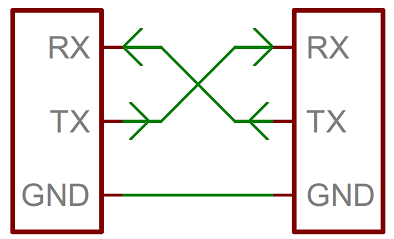
\includegraphics[width=0.5\linewidth]{imagenes/Uart}
	\caption{Comunicación UART}
	\label{fig:Comunicación UART}
\end{figure}


El UART/ACE convierte el bus paralelo interno de la computadora en un flujo de datos en serie. También proporciona el búfer de memoria de entrada y salida primero en entrar, primero en salir (FIFO), un reloj de interfaz (normalmente denominado generador de velocidad de transmisión), y señales de temporización y reconocimiento de la interfaz. La entrada y salida analógica del UART/ACE puede estar almacenada en búfer por un controlador de línea. La salida del DTE se conoce como la señal del transmisor (TX), mientras que la entrada se denomina la señal recibida (RX). El cable de la interfaz está limitado a una longitud máxima de 15 m. La longitud del cable determina la velocidad máxima de transmisión de datos que se puede usar de manera fiable en el bus de interfaz.


\subsection{SQL}
SQL. Structured Query Language (lenguaje de consulta estructurado), es un lenguaje surgido de un proyecto de investigación de IBM para el acceso a bases de datos relacionales. Actualmente se ha convertido en un estándar de lenguaje de bases de datos, y la mayoría de los sistemas de bases de datos lo soportan, desde sistemas para ordenadores personales, hasta grandes ordenadores. \\

\subsection{PHP MY ADMIN}
PhpMyAdmin es una herramienta de software gratuita escrita en PHP, destinada a manejar la administración de MySQL a través de la Web. phpMyAdmin admite una amplia gama de operaciones en MySQL y MariaDB. Las operaciones de uso frecuente (administración de bases de datos, tablas, columnas, relaciones, índices, usuarios, permisos, etc.) se pueden realizar a través de la interfaz de usuario, mientras aún tiene la capacidad de ejecutar directamente cualquier declaración SQL. \\
Características:

\begin{itemize}
 	\item Interfaz web intuitiva.
 	\item Soporte para la mayoría de las funciones de MySQL.
 	\item Examinar y soltar bases de datos, tablas, vistas, campos e índices.
 	\item Crear, copiar, eliminar, renombrar y modificar bases de datos, tablas, campos e índices.
	\item Servidor de mantenimiento, bases de datos y tablas, con propuestas de configuración del servidor.
	\item Ejecute, edite y marque cualquier instrucción SQL, incluso consultas por lotes.
	\item Administrar cuentas de usuario y privilegios de MySQL.
	\item Transformar los datos almacenados en cualquier formato utilizando un conjunto de funciones predefinidas, como mostrar datos BLOB como imagen o enlace de descarga.
 \end{itemize}

\subsection{AJAX}
AJAX es una técnica de de desarrollo WEB, por la cual se pueden crear aplicaciones WEB más rápidas y cómodas para el usuario. Por medio de esta técnica el cliente puede interactuar con el servidor de manera asincrónica, actualizando las páginas, sin necesidad de volver a cargarlas. Esta técnica, no solo es más cómoda y amigable para el usuario (ya que se asemeja a las aplicaciones de escritorio) sino que además es más rápida, porque cada vez que se necesita actualizar un dato en una página, no es necesario recargarla nuevamente (solo se recarga la sección necesaria de la misma). \\
Ventajas:

\begin{itemize}
 	\item Las páginas no se recargan constantemente.
 	\item El tiempo de espera es menor.
 	\item Se pueden lograr cosas que sin AJAX definitivamente no se podrían hacer, como el conocido Google Maps por ejemplo.
 \end{itemize}

Desventajas:
\begin{itemize}
 	\item Falta de integración con el botón "retroceder" de los navegadores. Esto se debe a que siempre estamos en la misma página (no la recargamos). Y algunas veces puede llegar a confundir al usuario.
 	\item Es necesario que el navegador soporte y tenga habilitado JavaScript. No es una gran desventaja, ya que casi todos los navegadores modernos soportan JavaScript.
 	\item Al tener que ejecutar más código del lado del cliente, puede enlentecerse el rendimiento de la máquina del cliente. Por eso debe usarse AJAX con moderación.
 	\item Al no recargar las páginas, y siempre estar en la misma, no se tiene una URL a la cual poder referirse, en caso de querer recomendar la página, o volver a esa página. Por eso debe saberse cuando usar AJAX y cuando no.
 \end{itemize}

\subsection{Servicio de Sigfox}
Partiendo del uso de este servicio, se tiene una tarjeta de desarrollo, en la cual se hace la programación para la captura de los datos de los sensores, una vez capturados son encapsulados para ser enviados al servidor propio de este servicio, el tamaño máximo del mensaje debe ser máximo de 12 bytes. A continuación se muestra como es que se hace la programación para la lectura de un sensor de temperatura en el IDE de Arduino, en el cual se incluye una librería de la tarjeta de desarrollo para enviar datos de una manera más sencilla, el programa consiste en la lectura de un sensor de temperatura el cual captura el dato, para después ser encapsulado y enviado, iniciando el payload y después encapsulando el dato a enviar, y finalmente se envía al servidor.

\begin{figure}
	\centering
	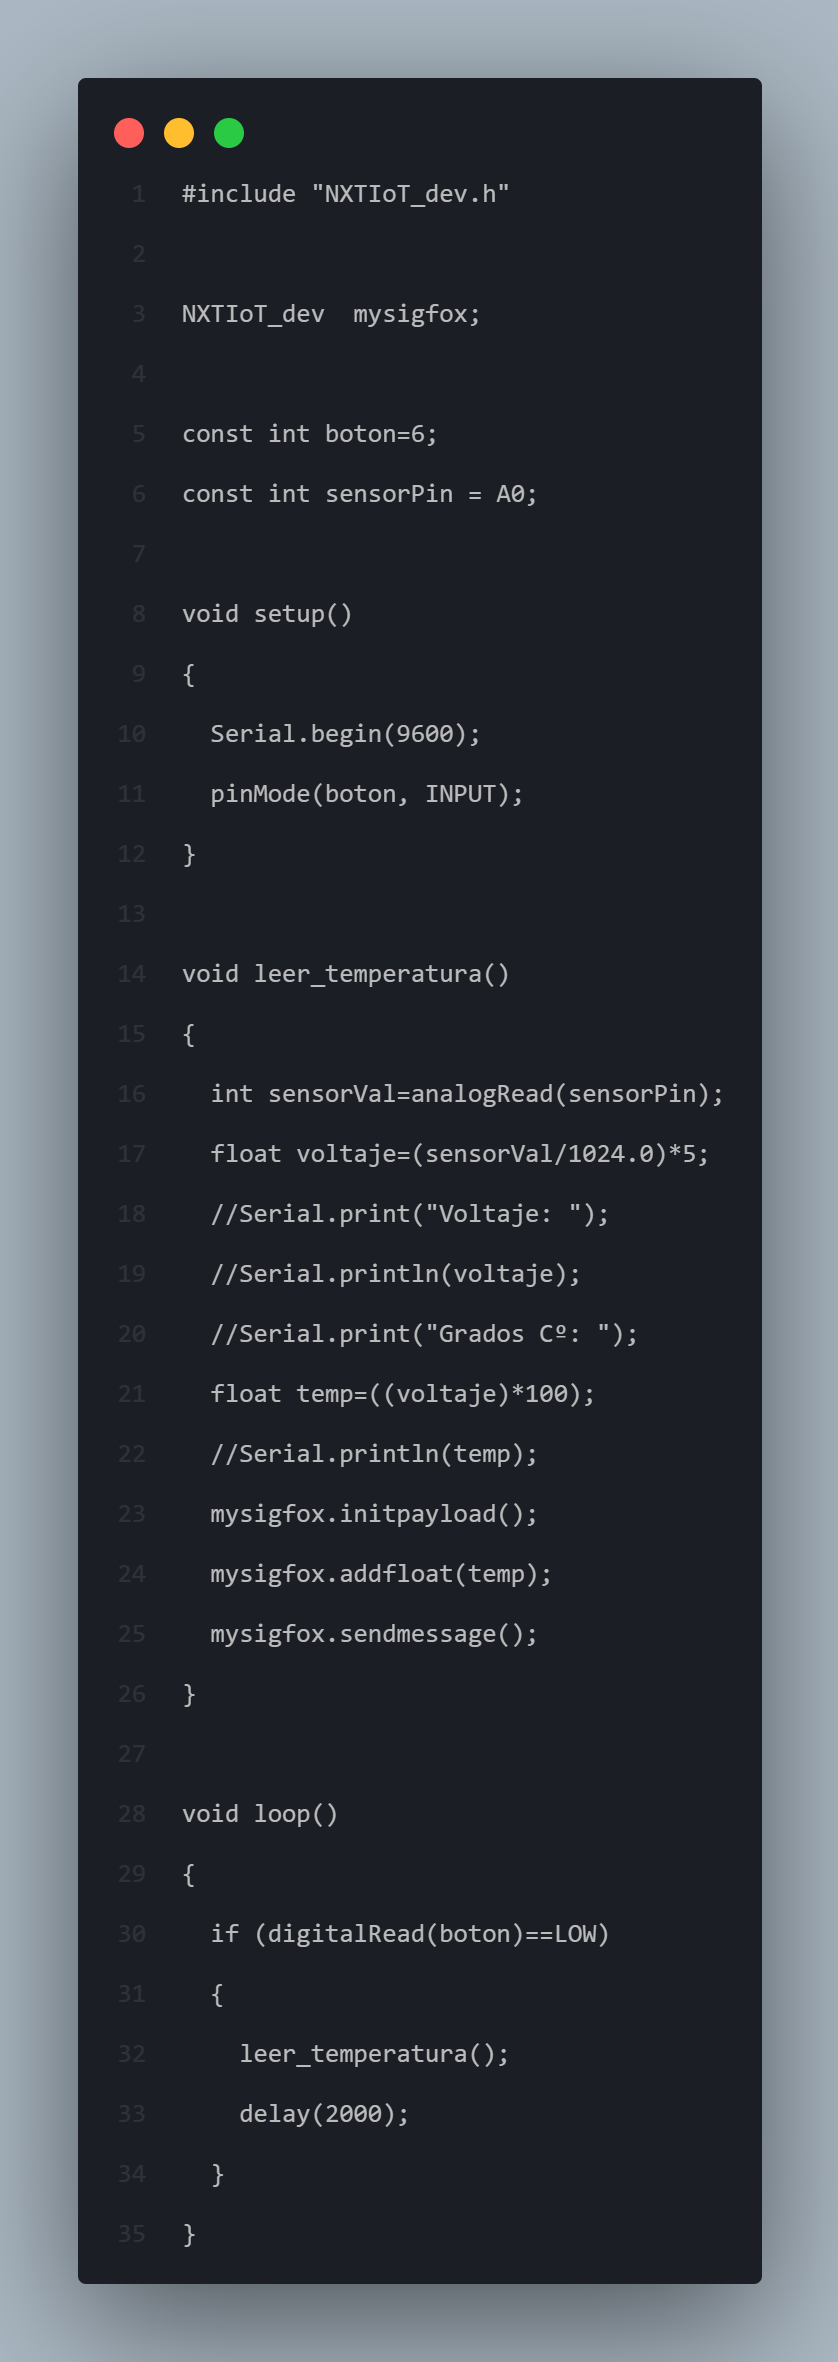
\includegraphics[width=0.7\linewidth, height=1\textheight]{imagenes/arduino}
	\caption{Lectura de sensor}
	\label{fig:Lectura de sensor}
\end{figure} 

\vspace{9cm}


Cuando los datos son enviados desde la tarjeta, son recibidos en el servidor de Sigfox, aquí se tiene que configurar los parámetros que se van a recibir, en este caso son 4 variables las que se van a manejar, por lo tanto, configuramos el tipo de dato y el nombre de la variable que va a tomar. \\

En el payload seleccionamos que será personalizado y pasamos a darle la configuración de los parámetros y el tipo de datos, en este caso se configuro de la siguiente manera: 
\textbf{temp::float:32:little-endian oxigen::uint:8 turbidez::uint:8 dioxido::uint:8}. \\
En lo cual estamos indicando que recibirá 4 variables diferentes, indicando si son enteros o flotantes. \\

\begin{figure}[h]
	\centering
	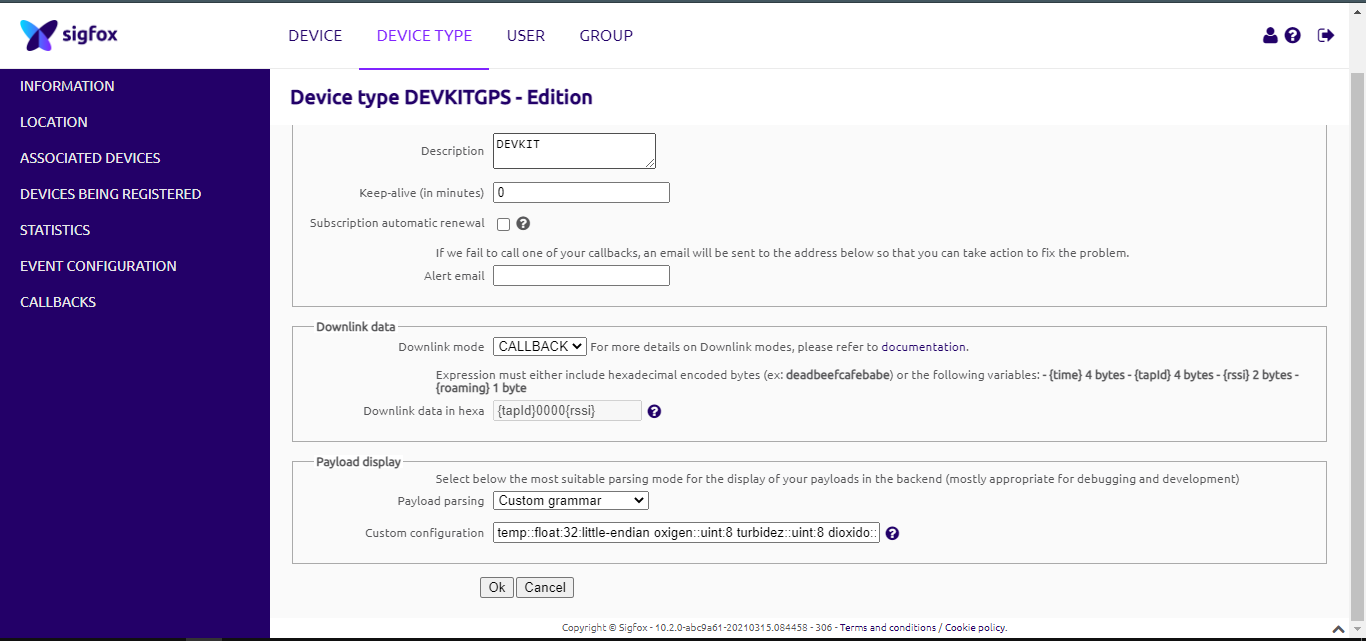
\includegraphics[width=1\linewidth]{imagenes/custom_grammar}
	\caption{Configuración del payload}
	\label{fig:Configuración del payload}
\end{figure}

Una vez configurado esto, en la sección de mensajes se podrá visualizar los mensajes que han sido enviados y los mostrara con sus respecticos datos, como se puede observar el mensaje encapsulado es descifrado y mostrado respectivamente como se configuro, especificando el dato la fehca y hora, el estado del callback y la localización. \\

\begin{figure}[t!]
	\centering
	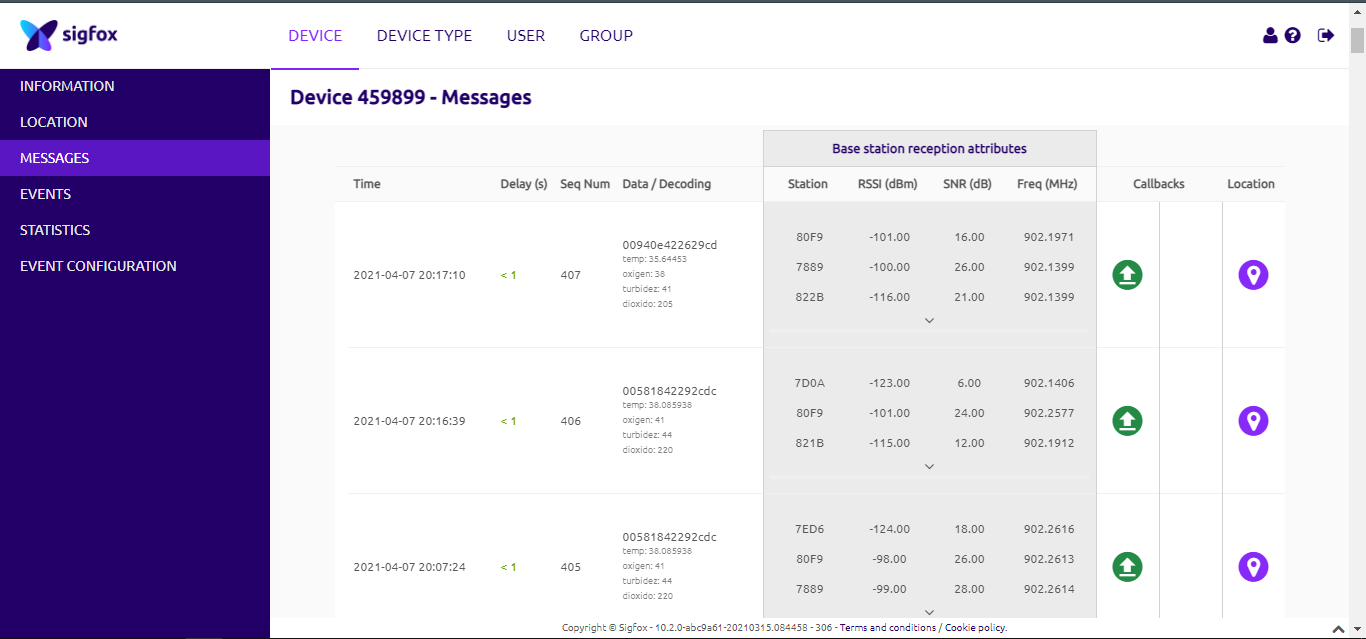
\includegraphics[width=1\linewidth]{imagenes/mensajes_sigfox}
	\caption{Mensajes en Sigfox}
	\label{fig:Mensajes en Sigfox}
\end{figure}

\vspace{5cm}


\subsubsection{Configuración del callback}
Para configurar el Callback y recibir los datos en nuestra aplicación hacemos la configuración, ingresando la URL del servidor donde se procesaran los datos y se almacenaran en una base de datos MySql, haciendo uso de PHP para la inserción de los datos recibidos desde Sigfox, primero configuramos el Callback, ingresando los parámetros que anteriormente se había configurado en el Payload, posteriormente se ingresa la URL en donde se harán las peticiones al servidor de nuestra aplicación web, haciendo una petición HTTP con el método POST, seguido en el cuerpo indicamos las variables que serán enviadas al servidor.

\begin{figure}[bh!]
	\centering
	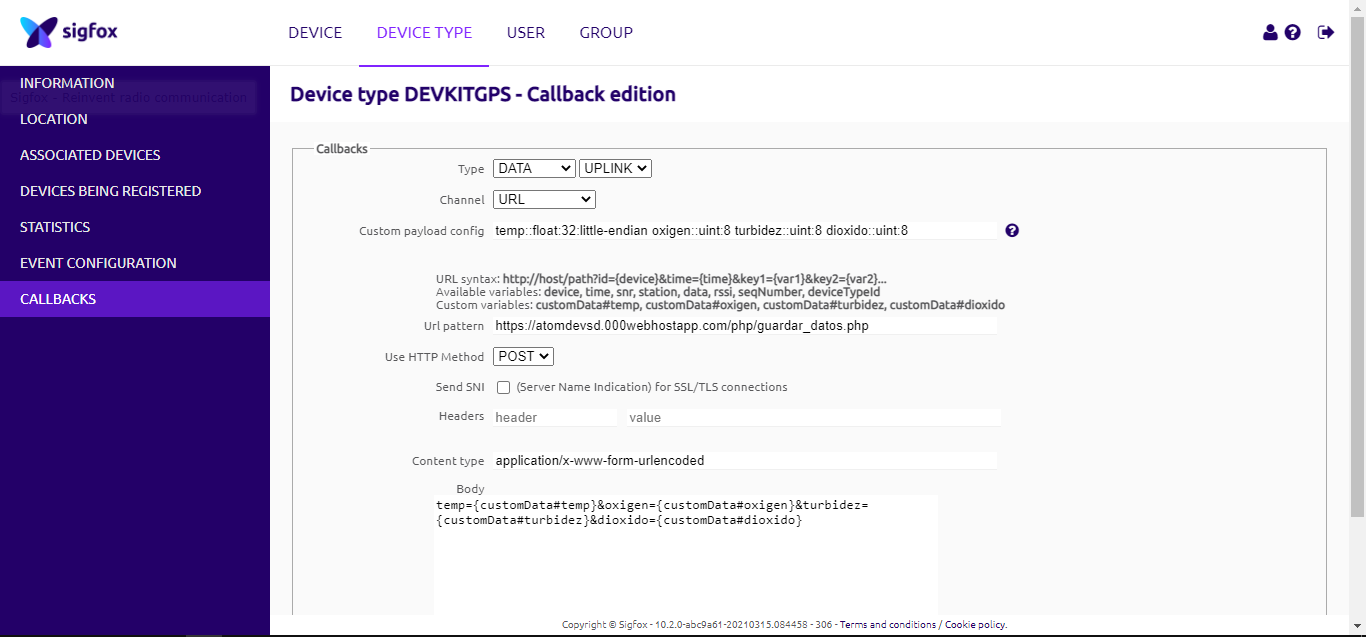
\includegraphics[width=0.8\linewidth]{imagenes/callback}
	\caption{Configuración del Callback}
	\label{fig:Configuración del Callback}
\end{figure}

\subsection{Diagrama de comunicación}

En este diagrama se puede ver de forma visual, como es la comunicación entre la boya con el sistema de sensores y la tarjeta para el envío de mensajes y coordenadas, para ello se hace uso de los puertos UART para transmitir los datos tomados de los sensores y procesarlos para que sean enviados a la aplicación, donde podrá visualizarlos el usuario, para tomar las coordenadas del módulo GPS también se hace uso del puerto UART para que la tarjeta reciba las coordenadas que esta tomando el GPS, y sean enviados a la nube y visualizados en la aplicación web. 

\begin{figure}[h]
	\centering
	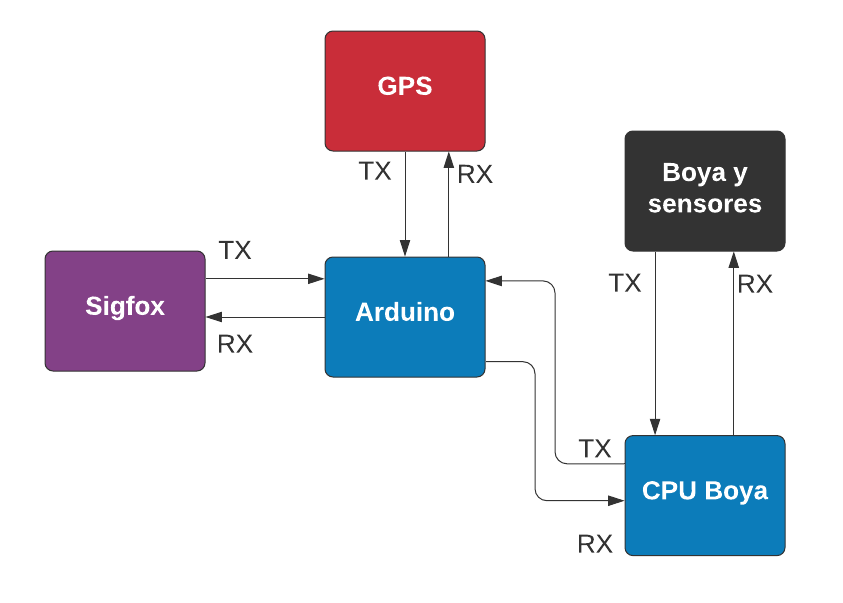
\includegraphics[width=0.8\linewidth]{imagenes/diagramaBoya}
	\caption{Diagrama de comunicación entre la boya y la tarjeta de desarrollo}
	\label{fig:Diagrama de comunicación entre la boya y la tarjeta de desarrollo}
\end{figure}

\begin{figure}[h]
	\centering
	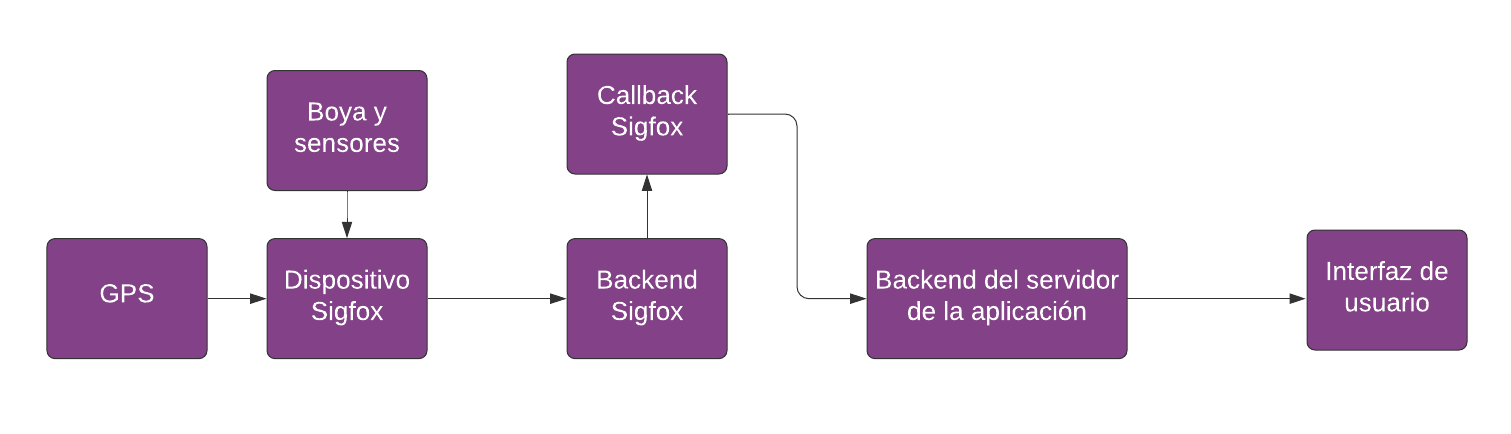
\includegraphics[width=0.8\linewidth]{imagenes/arquitecturaProyecto}
	\caption{Diagrama de comunicación del proyecto}
	\label{fig:Diagrama de comunicación del proyecto}
\end{figure}

\vspace{1cm}

\subsection{Aplicación web}
Para la aplicación web en donde se mostrará al usuario de forma grafica los datos que son enviados y capturados desde la tarjeta, se diseño una base de datos en MySql en la cual, los datos enviados recibidos en el servidor de Sigfox, son enviados también al servidor de la aplicación para ser guardados en la base de datos propia.

\subsubsection{Base de datos}

Para que los datos sean guardados en la base de datos, son enviados desde el servidor de Sigfox, en donde anteriormente se hizo la configuración del Callback para que los datos sean enviados y recibidos en el servidor de la aplicación, usando PHP para recibir dichos datos y almacenados en la base de datos.

La base de datos se compone de dos tablas:
\begin{itemize}
	\item Tabla de mensajes.
	\item Tabla de usuarios.
\end{itemize}

\subsubsection{Tabla de mensajes}

En la tabla, es la principal tabla de la base de datos en mostrar la información al usuario, aquí es donde recibe los datos leídos desde la tarjeta de desarrollo y enviados desde el Callback programado desde el servicio de Sigfox, recibe los 4 parámetros principales que son con los que cuenta el sistema de sensores: Oxigeno, temperatura, turbidez y dióxido de carbono, también hay una columna con la fecha y hora en que se recibió el mensaje, esto ayuda para tener un control en el historial de la aplicación para hacer una búsqueda de alguna fecha en especifico cuando se requiera.

\begin{figure}[h!]
	\centering
	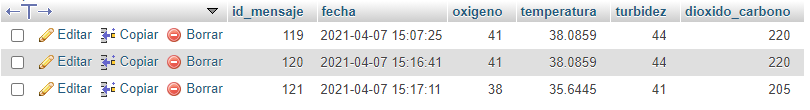
\includegraphics[width=0.8\linewidth]{imagenes/dbmensajes}
	\caption{Tabla de mensajes.}
	\label{fig:Tabla de mensajes}
\end{figure}

\begin{figure}[h!]
	\centering
	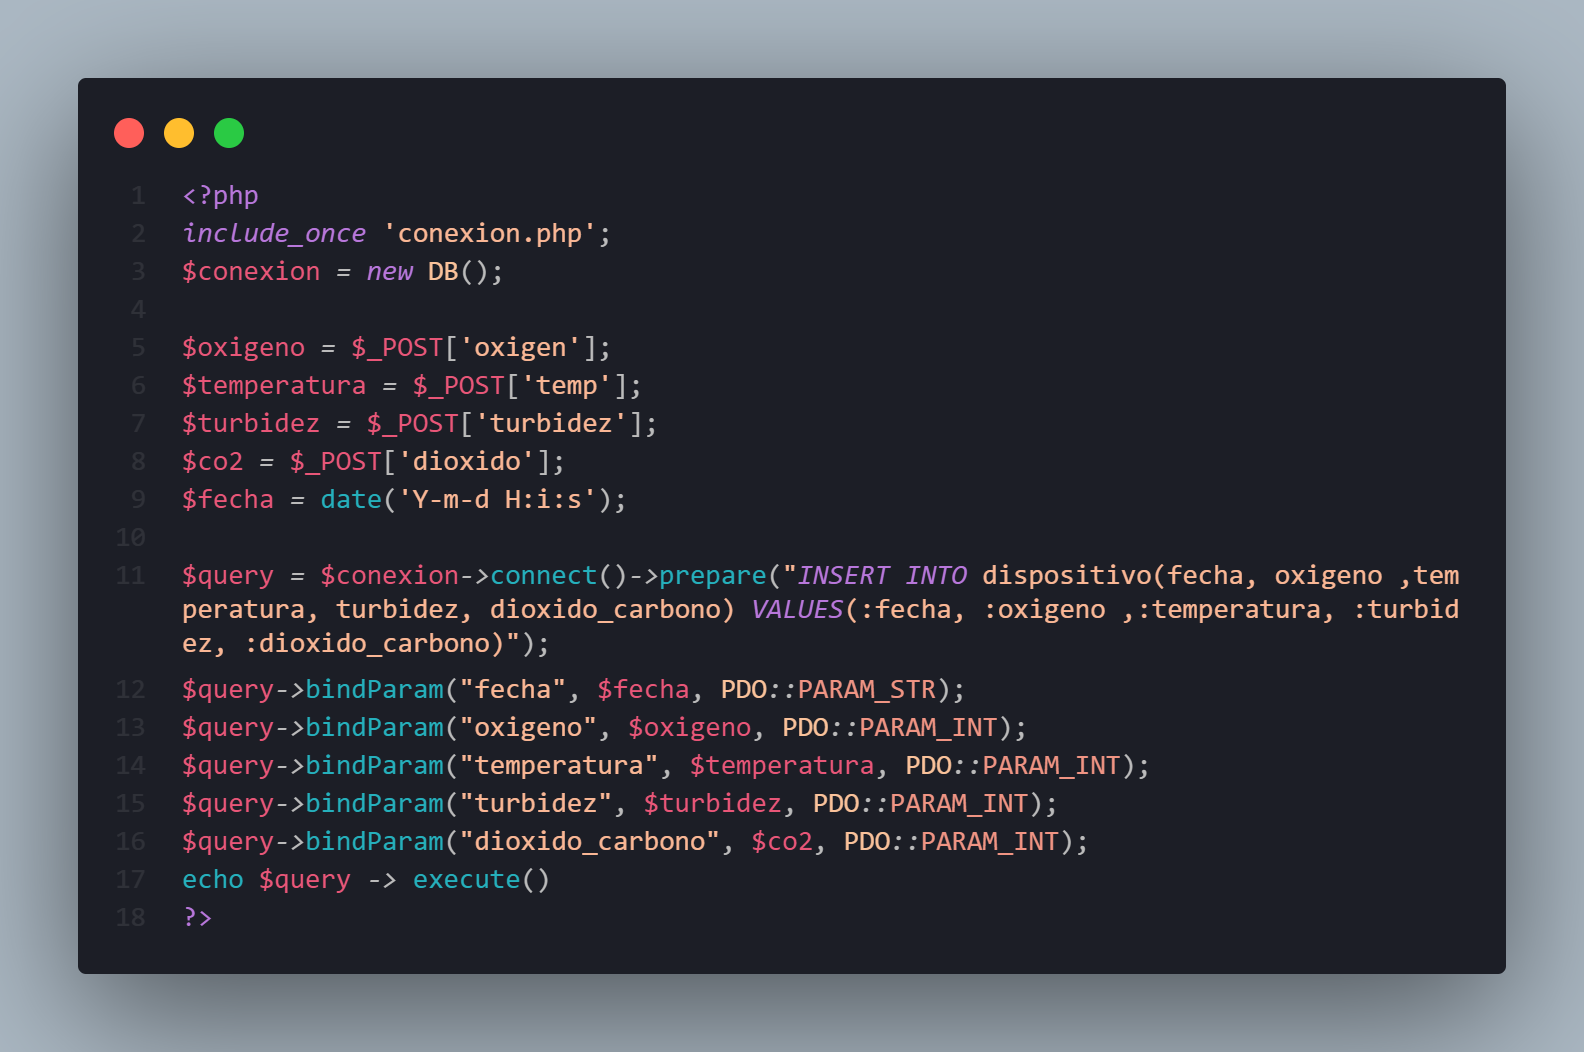
\includegraphics[width=0.8\linewidth]{imagenes/guardar_datos}
	\caption{Guardando los datos enviados desde Sigfox con PHP}
	\label{fig:Guardando los datos enviados desde Sigfox con PHP}
\end{figure}

\vspace{5cm}


\subsubsection{Tabla de usuarios}
En esta tabla no hace nada mas que almacenar al usuario de administrador, el cual será el que tendrá acceso a la aplicación para la recopilación de datos.

\begin{figure}[h!]
	\centering
	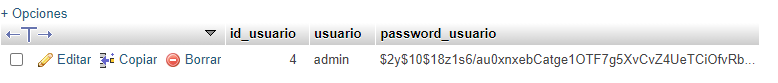
\includegraphics[width=0.8\linewidth]{imagenes/dbusuario}
	\caption{Tabla de usuarios.}
	\label{fig:Tabla de usuarios}
\end{figure}

\begin{figure}[h!]
	\centering
	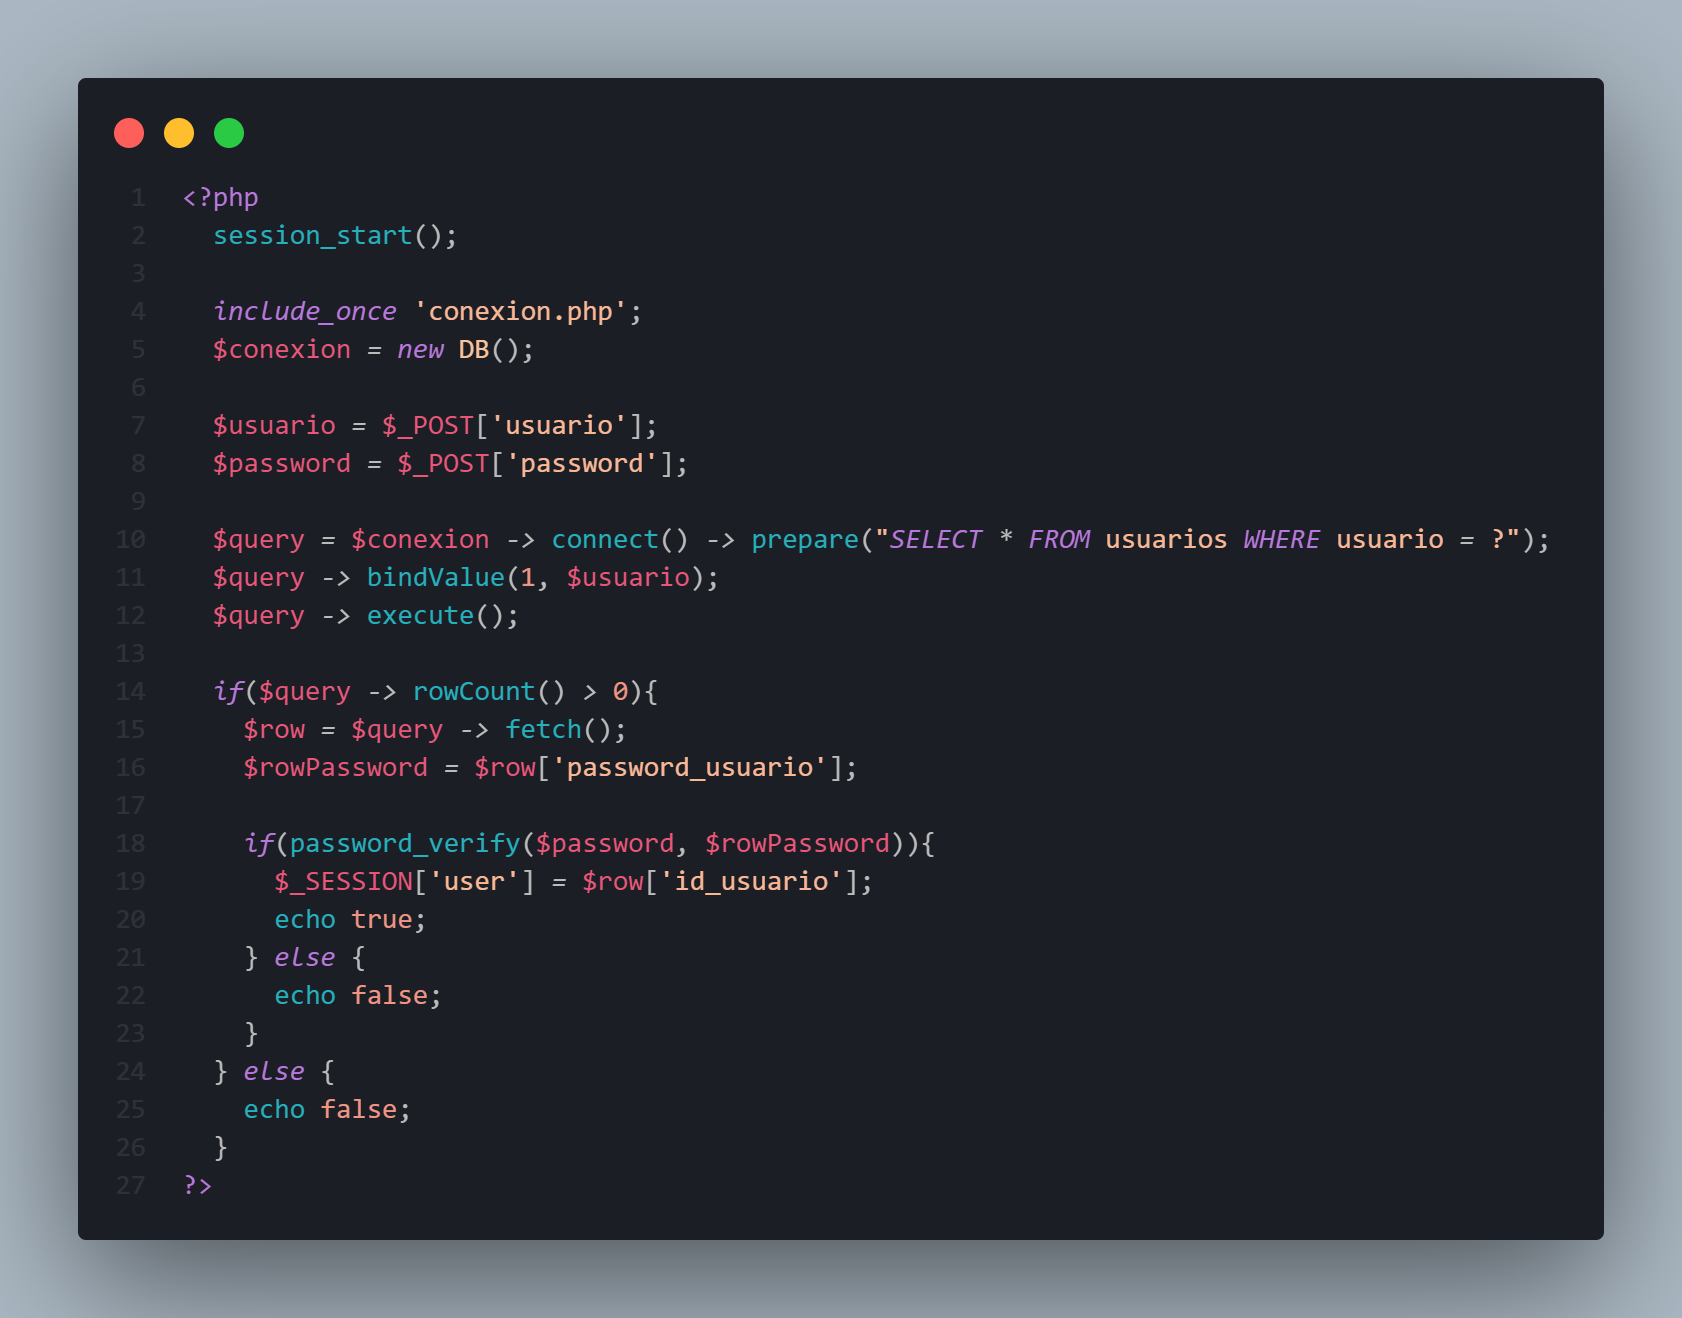
\includegraphics[width=0.8\linewidth]{imagenes/phplogin}
	\caption{Validación para el inicio de sesón con PHP}
	\label{fig:Validación para el inicio de sesón con PHP}
\end{figure}

\vspace{10cm}

\subsubsection{Tabla de coordenadas}
En esta tabla no hace nada más que almacenar las coordenadas que son enviadas desde el dispositivo que lee el módulo GPS, para obtener la latitud y longitud.

\begin{figure}[h]
	\centering
	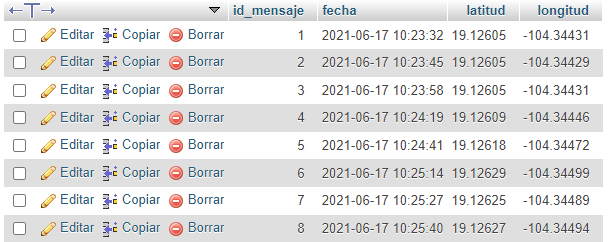
\includegraphics[width=0.8\linewidth]{imagenes/dbcoordenadas}
	\caption{Coordenadas}
	\label{fig:Coordenadas}
\end{figure}


\vspace{8cm}

\subsubsection{Interfaz del usuario}
La aplicación consiste en 3 secciones, en las cuales se muestra de forma gráfica y especifica los datos tomados y enviados desde la tarjeta de desarrollo con Sigfox, y un inicio de sesión para tener el control de quien tenga acceso al sistema.

\subsubsection{Inicio de sesión}
Esta es la vista principal de la aplicación, el usuario registrado es el único que tendrá acceso a la aplicación para la visualización de datos, de otra manera no se puede acceder a la pagina principal una vez iniciada la sesión.

\begin{figure}[h!]
	\centering
	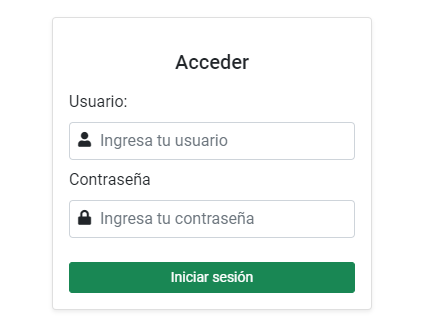
\includegraphics[width=0.5\linewidth]{imagenes/login}
	\caption{Inicio de sesión}
	\label{fig:Inicio de sesión}
\end{figure}

\vspace{3cm}



\subsubsection{Pagina principal}
En la pagina principal de la aplicación, una vez que el usuario haya iniciado sesión, se tiene un menú de navegación superior, en el cual muestra al usuario que inicio sesión y a darle clic podrá cerrar la sesión, después se puede observar en la parte inferior cuatro secciones dentro de esta página, en la cual se muestra mediante graficas las diferentes variables que se leen desde los sensores, partiendo del lado derecho, se obtiene el ultimo dato enviado desde la tarjeta, y en la parte derecha se muestra la gráfica de esa variable en específico mostrando los valores y la hora en que fueron enviados, también se tiene la opción de buscar mediante fecha en la gráfica, para así tener un historial de los datos que han sido enviados en la fecha especificada.

\subsubsection{Gráfica de oxigeno}

\begin{figure}[h!]
	\centering
	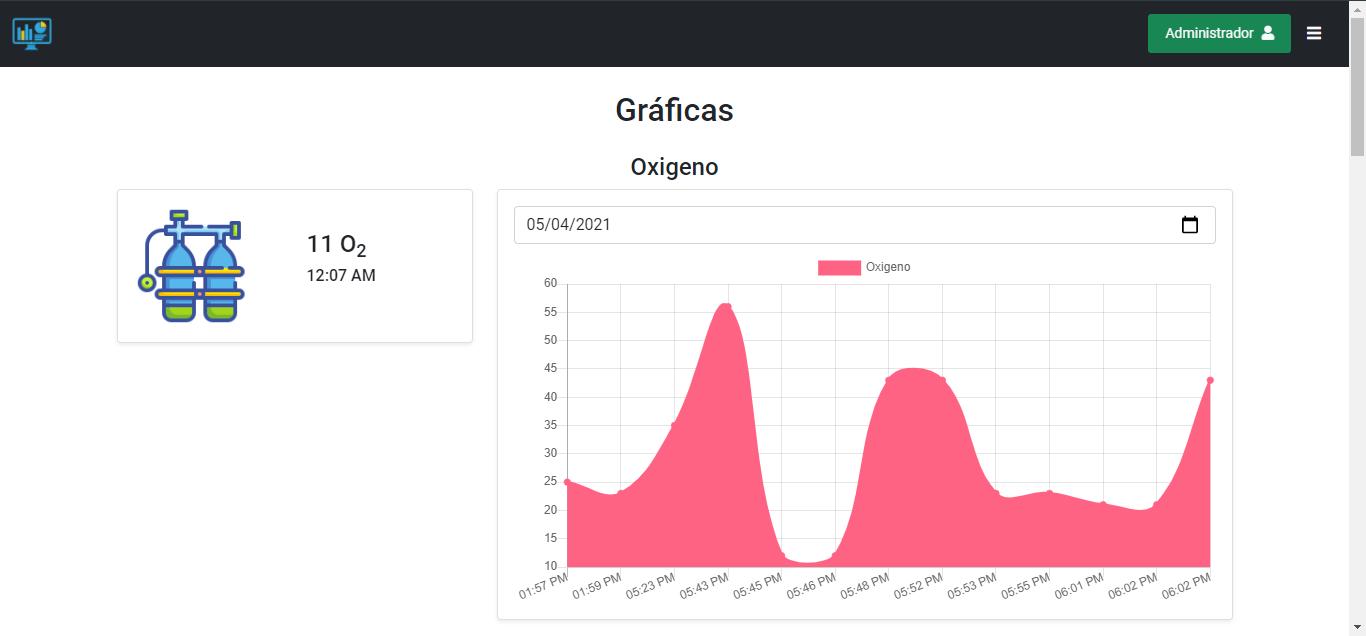
\includegraphics[width=0.8\linewidth]{imagenes/oxigenoGrafica}
	\caption{}
	\label{fig:oxigenografica}
\end{figure}

\subsubsection{Gráfica de temperatura}

\begin{figure}[h!]
	\centering
	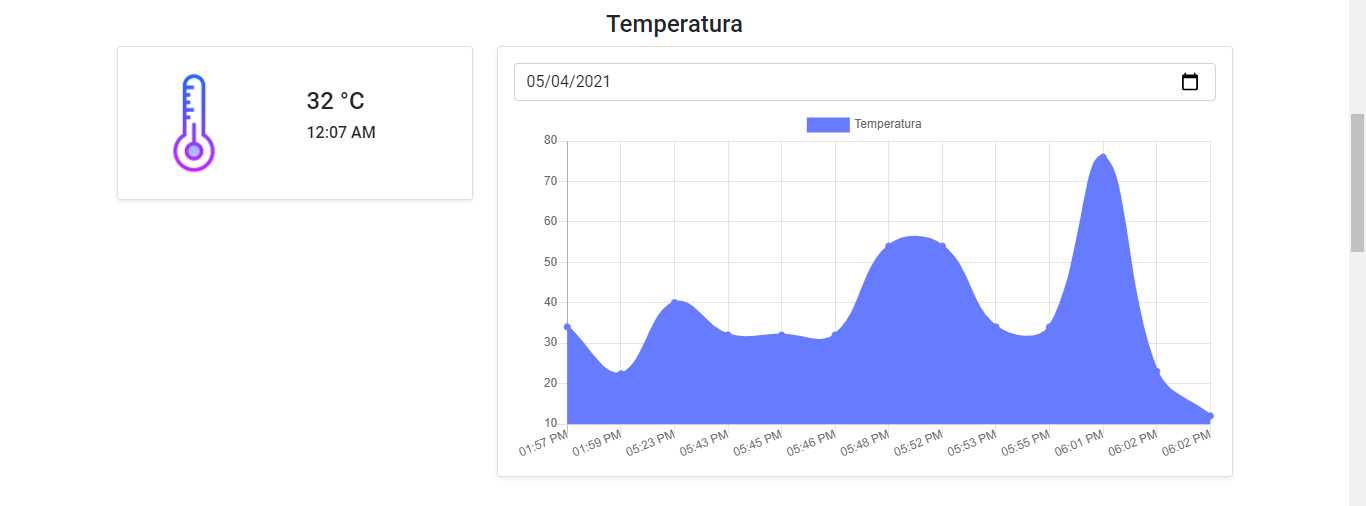
\includegraphics[width=0.7\linewidth]{imagenes/temperaturaGrafica}
	\caption{Gráfica de temperatura}
	\label{fig:Gráfica de temperatura}
\end{figure}

\subsubsection{Gráfica de turbidez}

\begin{figure}[h!]
	\centering
	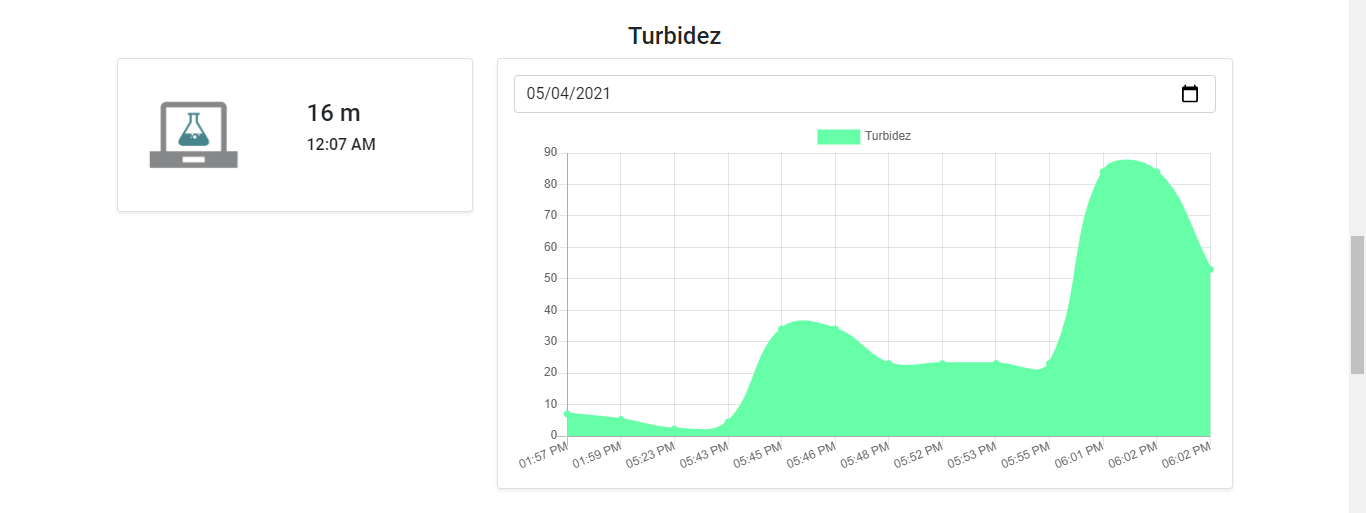
\includegraphics[width=0.7\linewidth]{imagenes/turbidezGrafica}
	\caption{Gráfica de turbidez}
	\label{fig:Gráfica de turbidez}
\end{figure}

\subsubsection{Gráfica de dióxido de carbono}

\begin{figure}[h!]
	\centering
	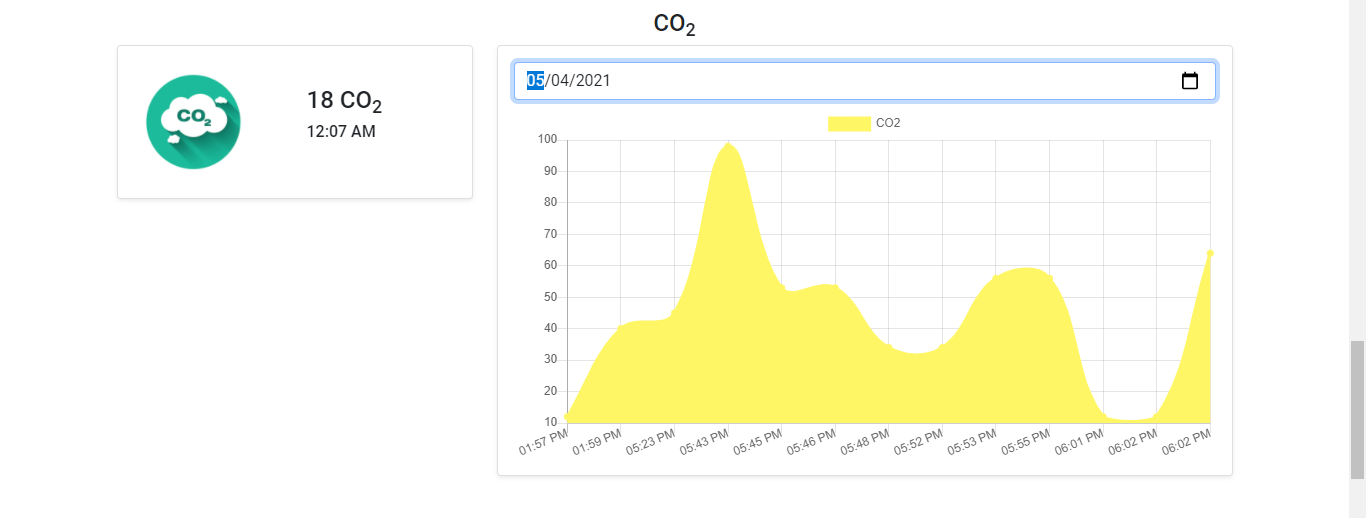
\includegraphics[width=0.7\linewidth]{imagenes/co2Grafica}
	\caption{Gráfica de dióxido de carbono}
	\label{fig:Gráfica de dióxido de carbono}
\end{figure}

\subsubsection{Tabla de variables registradas}

Para esta sección de la aplicación, se mostrara al usuario una tabla, la cual mostrara los datos que se han enviado desde el dispositivo, incluyendo la fecha y hora en el que fue recibido el mensaje así como también, las coordenadas para saber en que punto se encuentra ubicado el dispositivo, esto para llevar un historial de datos para que sea proporcionado al usuario cuando se requiera, buscando por fechas para obtener datos en especifico de la fecha seleccionada, también se tiene una opción para exportar la tabla a Excel, lo cual se podrá tener un respaldo en caso de necesitarlo al momento que se desee.

\begin{figure}[h]
	\centering
	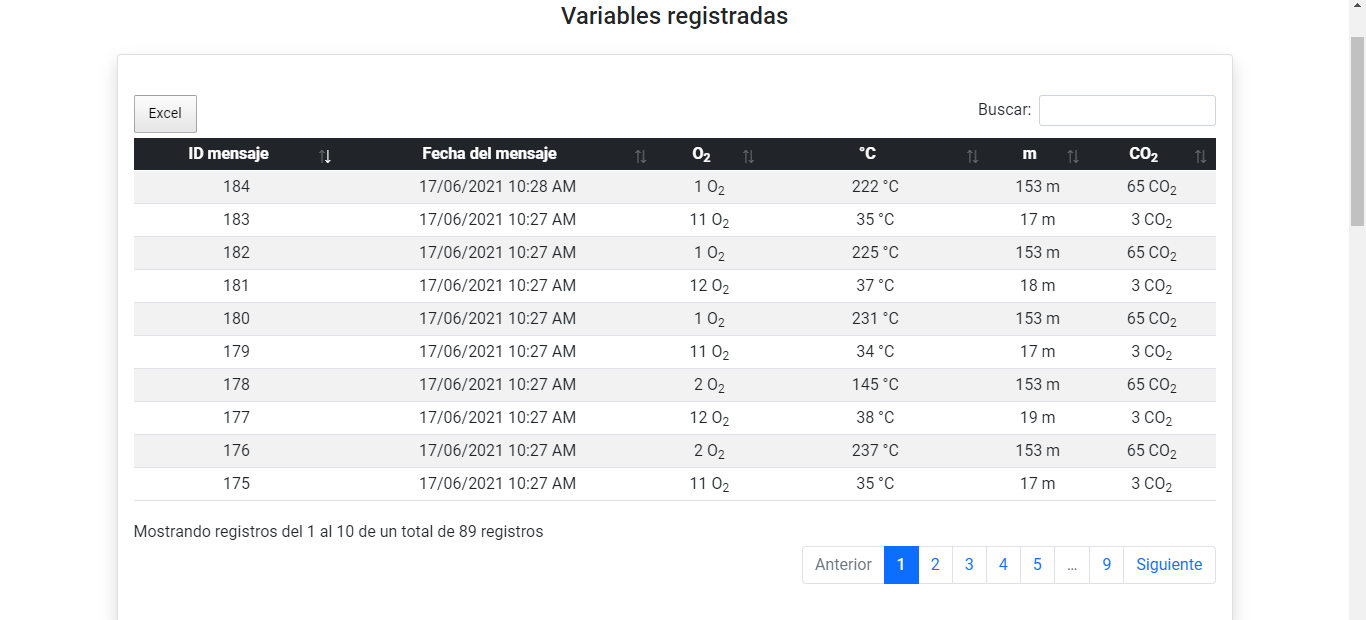
\includegraphics[width=0.8\linewidth]{imagenes/tablaVariables}
	\caption{Tabla de datos}
	\label{fig:Tabla de datos}
\end{figure}

\begin{figure}[h]
	\centering
	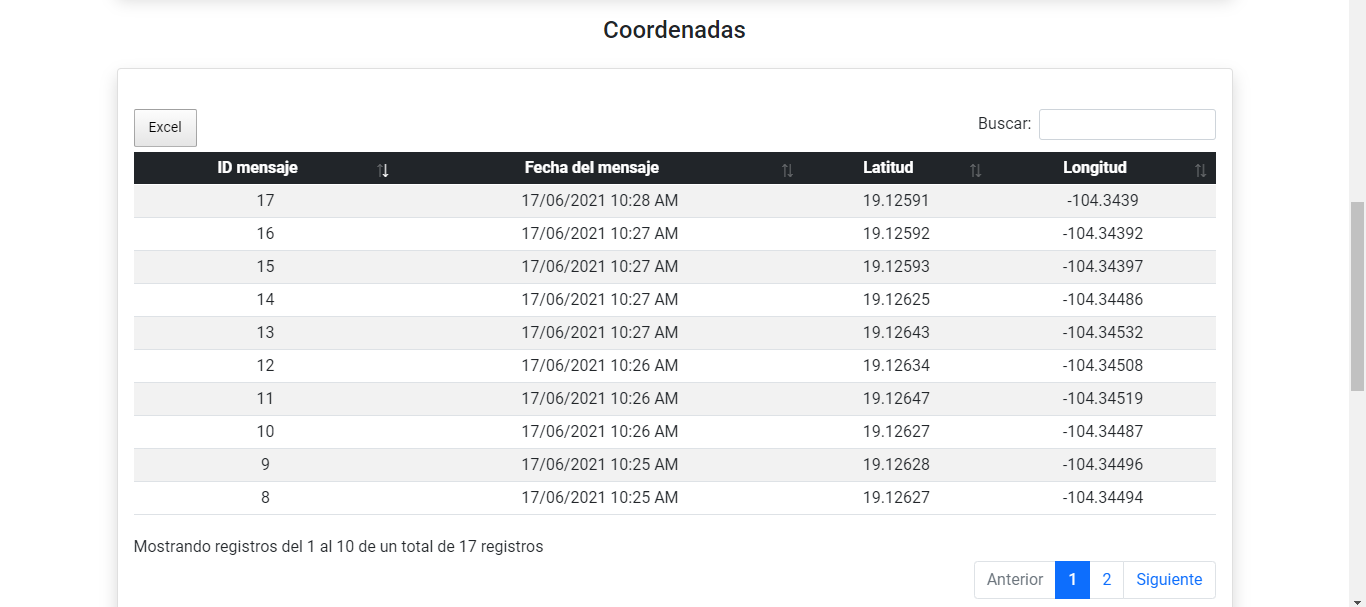
\includegraphics[width=0.8\linewidth]{imagenes/tablaCoordenadas}
	\caption{Tabla de coordenadas}
	\label{fig:Tabla de coordenadas}
\end{figure}

\vspace{5cm}


Al momento de exportar la tabla desde la aplicación, se descargará un archivo en Excel para la visualización de los datos.

\begin{figure}[h!]
	\centering
	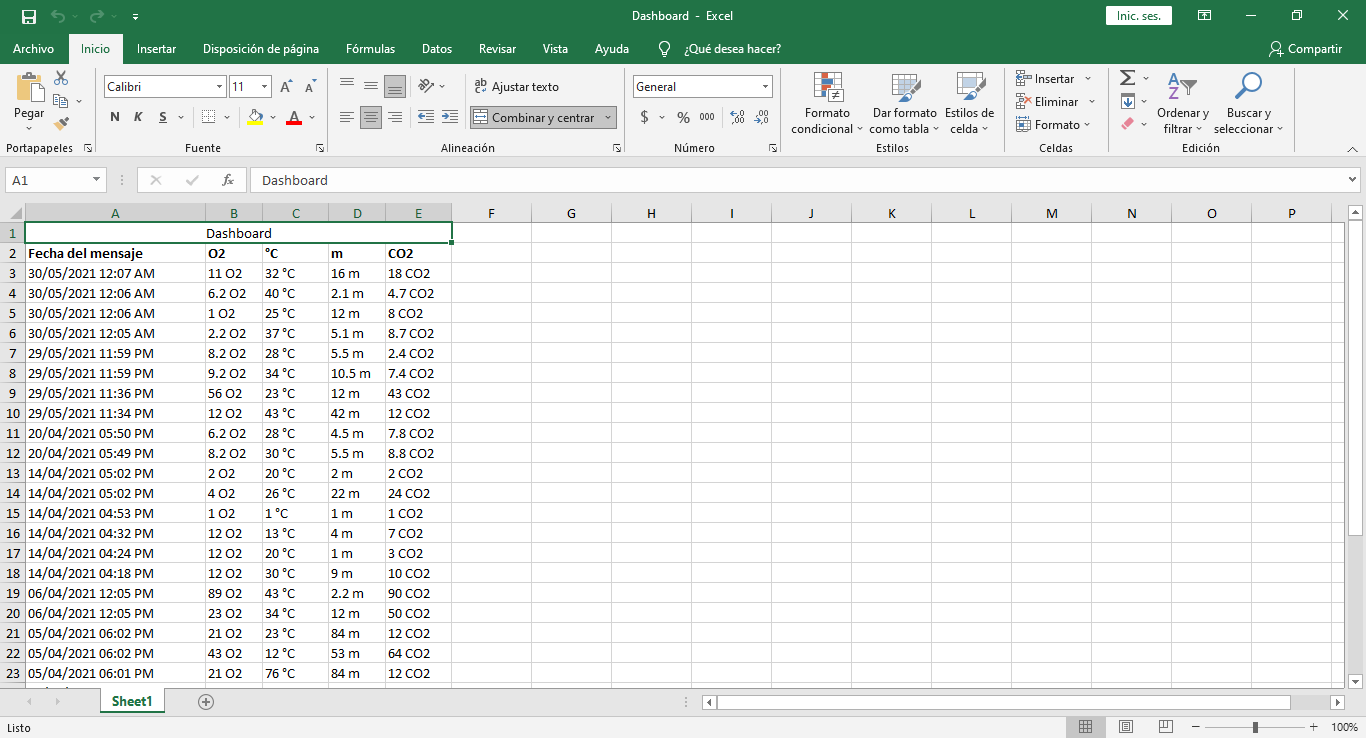
\includegraphics[width=0.8\linewidth]{imagenes/excel}
	\caption{Tabla en Excel}
	\label{fig:Tabla en Excel}
\end{figure}

\vspace{5cm}

\subsubsection{Geolocalización}

Para la geolocalización se consume una API de Google Maps para poder visualizar la ubicación del dispositivo en la aplicación, tomando las coordenadas enviadas desde el dispositivo conectado a la boya, en el módulo GPS que tiene integrado, tomando como referencia la latitud y longitud para poder mostrar un marcador en el mapa.

\begin{figure}[h!]
	\centering
	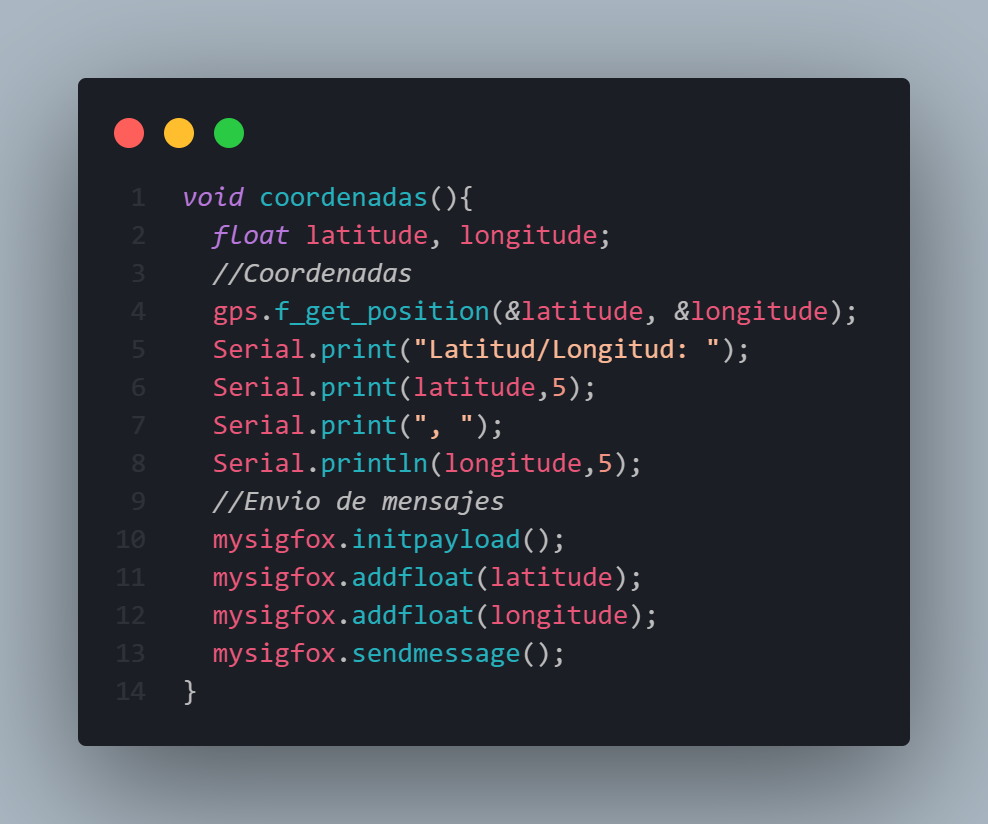
\includegraphics[width=0.7\linewidth]{imagenes/coordenadasArduino}
	\caption{Obtención de coordenadas con el módulo GPS}
	\label{fig:Obtención de coordenadas con el módulo GPS}
\end{figure}

\begin{figure}[h!]
	\centering
	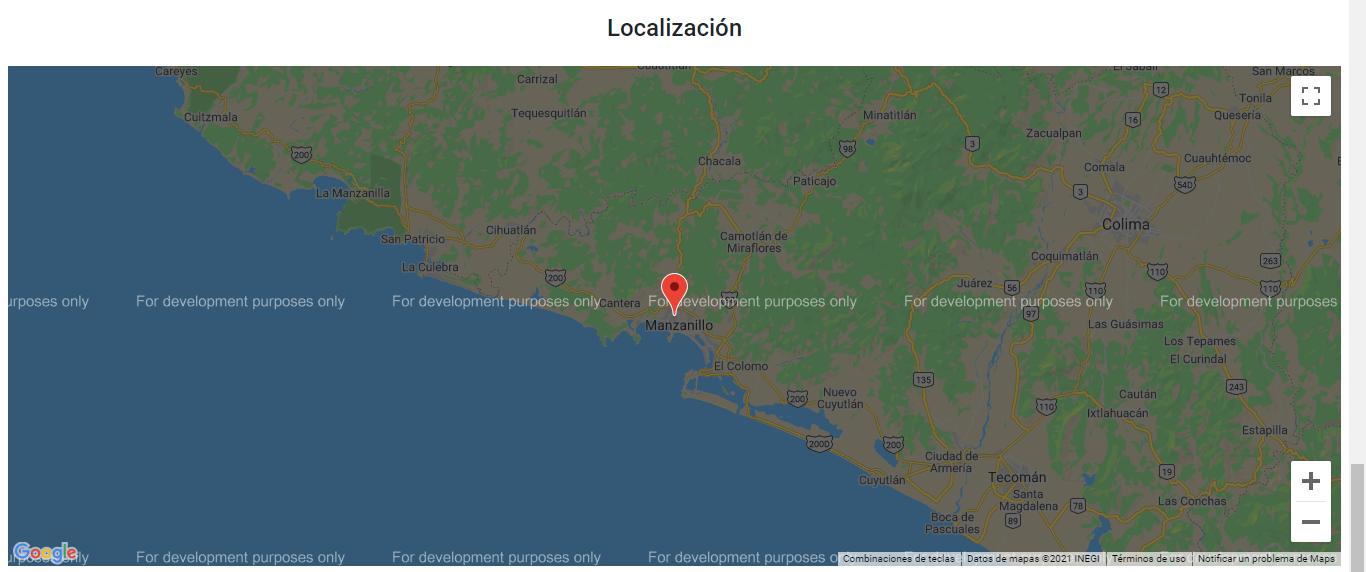
\includegraphics[width=0.7\linewidth]{imagenes/localizacion}
	\caption{Localización}
	\label{fig:Localización}
\end{figure}


Debido a la pandemia del Coronavirus que empezó desde marzo del año 2020 hasta el presente año 2021, no fue posible acceder al plantel de FACIMAR en donde se encuentra la boya y el sistema de sensores para trabajar en base a ello, debido al problema antes mencionado, por ello y para no atrasarnos en el proyecto de tesis para el fin de carrera, se tomó la decisión junto con el asesor de tesis de optar por una simulación, simulando la toma de las 4 variables como si fueran las tomadas del sistema de sensores que tiene integrado la boya, ya que no fue posible trabajar de manera presencial con ellos, así, simulando la lectura de las variables mediante un circuito de potenciómetros, para que sean leídos con la tarjeta de desarrollo y enviados al servidor para que sean mostrados en la aplicación que se desarrolló, sin perder de vista el principal problema a resolver, el cual es hacer uso de tecnología Sigfox, la cual reduce costos y consumo de energía para el uso de IoT y se adapta adecuadamente a este tipo de proyectos, ya que anteriormente la boya contaba con una red satelital, lo cual implica mayores costos del servicio y mayor consumo de energía pero con una cobertura mayor, en este caso el servicio de Sigfox ofrece una buena cobertura en el municipio de Manzanillo hasta de 30 KM y mar a dentro, lo cual es buena cobertura ya que la boya no está a más de 5 KM de la costa. \\

El acceso a la aplicación esta disponible en el siguiente link: \\
\underline{https://atomdevsd.000webhostapp.com/index.php} \\
Con usuario: admin y contraseña: admin.







\bibliographystyle{apalike}
\begin{thebibliography}{n}
	\bibitem{holbox}
	Boya Holbox-México \\
	https://www.biodiversidad.gob.mx/pais/mares/simar/sidmo/boyasmex/holbox.html	
	\bibitem{Tboyas}
	[Martín Castaño Sánchez, 2011] Martín Castaño Sánchez (2011).Sistema de monitorización y supervisión de una boya de energía undimotriz. 
	\bibitem{Sigfox}
	Sigfox 	https://www.sigfox.com/en
	\bibitem{IoT}
	L. Atzori, A. Iera, and G. Morabito, ‘‘The Internet-of-Things: A survey,’’Comput. Netw., vol. 54, no. 15, pp. 2787–2805, 2010.
	\bibitem{UIoT}
	M. C. Domingo, ‘‘An overview of the Internet of underwater things,’’
	J. Netw. Comput. Appl., vol. 35, no. 6, pp. 1879–1890, 2012.
	\bibitem{Desafios}
	C.-C. Kao, Y.-S. Lin, G.-D. Wu, and C.-J. Huang, ‘‘A comprehensive study
	on the Internet of underwater things: Applications, challenges, and channel models,’’ Sensors, vol. 17, no. 7, p. 1477, 2017.
\end{thebibliography}

\end{document}